%Bibliographystyle wählen, Standard numeric
%\PassOptionsToPackage{style=apa}{biblatex}  %weitere Möglichkeiten siehe biblatex.pdf
\documentclass[12pt,DIV=15,BCOR=15mm,twoside,headsepline,abstract=true,listof=totoc,bibliography=totoc]{scrreprt}

%%%%%%%%%%%%%%%%%%%%%%%%%%%%%%%%%%%%%%%%%%%%%%%%%%%%%%%%%%%
%%%%%%%%%%%%% Uni Rostock Thesis Style %%%%%%%%%%%%%%%%%%%%
%%% bei Problemen, Mail an susann.dittmer@uni-rostock.de
%%%%%%%%%%%%%%%%%%%%%%%%%%%%%%%%%%%%%%%%%%%%%%%%%%%%%%%%%%%
% enthält schon viele wichtige Pakete
\usepackage[mnf]{thesis_uro} %Fakultät wählen: uni (Standard),inf,msf,ief,mnf,mef,juf,wsf,auf,thf,phf
\usepackage{pdflscape}
\usepackage[toc,page]{appendix}
\usepackage{siunitx}


\newtheorem{remark}{Bemerkung}[chapter]
\addbibresource{literatur.bib} %Bibliographiedateien laden

%Definition von Umgebungen
\newtheorem{kor}{Korollar}
\newtheorem{hsatz}{Hilfssatz}
\newtheorem{satz}{Satz}
\newtheorem{prop}{Proposition}
\newtheorem{defi}{Definition}
\newtheorem{lem}{Lemma}
\newtheorem{annahme}{Annahme}
\newtheorem{problem}{Problem}
\theoremstyle{remark}    %Styleänderung (Text aufrecht, ...)
\newtheorem{bem}{Bemerkung}
\newtheorem{bsp}{Beispiel}

%Beispiel für eigene Kommandos
\newcommand{\ol}{\overline} %Kurzform für \overline definiert 

% Daten für die Titelseite
\institut{Institut für Mathematik} %auskommentieren, wenn nicht benötigt
\arbeit{Bachelorarbeit}    %Praktikumsbericht
%Masterarbeit
%Abschlussarbeit (wenn Staatsexamensarbeit geschrieben wird - man kann dann, z.\,B. bei Untertitel "Wissenschaftliche Abschlussarbeit\\ im Rahmen  des Ersten Staatsexamens" eintragen)
%Bachelorarbeit
\autor{Hans-Hauke Haufe}
\betreuerGutachter{Dr. rer. nat. Tobias Strauß  \newline Universität Rostock\newline Mathematisch-Naturwissenschaftliche Fakultät} %hier \newline als Zeilenwechsel, da Tabelle mit \parbox im Hintergrund
\gutachter{Arne Pointeck \newline Fraunhofer-Institut für Großstrukturen in der Produktionstechnik IGP \newline Messtechnik}    
\date{21.09.2025}
\matrNr{2222\,0976}
\titel{Rekonstruktion und Tracking in dynamischen Umgebungen}
\untertitel{Maskenbasierte Anpassungen mithilfe eines Problem spezifisch trainierten Segmentierungsmodells} %auskommentieren, wenn nicht benötigt

\begin{document}
    \hypersetup{pageanchor=false}
    \begin{titlepage}
        \mytitle   %hier werden Daten für die Titelseite gesetzt
    \end{titlepage}

    \pagenumbering{Roman}
    \tableofcontents % Inhaltsverzeichnis

    \hypersetup{pageanchor=true}
    \pagenumbering{arabic}

    \chapter*{Abkürzungsverzeichnis}
    \addcontentsline{toc}{chapter}{Abkürzungsverzeichnis}
    \begin{acronym}
        \acro{SLAM}{Simultaneous Localization and Mapping}
        \acro{RGB-D}{Red-Green-Blue plus Depth}
        \acro{vSLAM}{visual SLAM}
        \acro{TSDF}{Truncated Signed Distance Field}
        \acro{ICP}{Itarativ Closest Point}
        \acro{SfM}{Structrue from Motion}
        \acro{RPE}{Realtive Pose Error}
        \acro{ATE}{Absolute Trajectory Error}
        \acro{P2P}{Point to Plane}
        \acro{CNN}{Convolutional Neural Network}
        \acro{FCN}{Fully Convolutional Network}
        \acro{ASPP}{Atrous Spatial Pyramid Pooling}
        \acro{GIS}{Genric Image Segmentation}
        \acro{PIS}{Promtable Image Segmentation}
        \acro{TPE}{Tree-Structrue Parzen Estimator}
        \acro{IoU}{Intersection over Union}
        
    \end{acronym}
    \chapter{Einleitung}
    In modernen Milchviehbetrieben spielt die präzise Fütterung eine entscheidende Rolle für Tiergesundheit, Milchleistung und Ressourceneffizienz. Eine Möglichkeit, 
    die Fütterung zu optimieren, sowie Tiergesundheit zu überwachen, ist die regelmäßige und genaue Messung der verbleibenden Futtermenge im Stall.
    Die manuelle Erfassung ist jedoch zeitaufwendig, fehleranfällig und auch nicht ununterbrochen möglich. Automatisierte Verfahren können hier unterstützen, insbesondere 
    Systeme, die das Futtervolumen räumlich erfassen und auswerten.\\\\
    Die räumliche Rekonstruktion in einem Stall mit frei bewegenden Kühen ist technisch anspruchsvoll. Kühe bewegen sich unvorhersehbar, verdecken Teile der Futterfläche 
    und verändern die Szene kontinuierlich. Klassische 3D-Mapping-Algorithmen setzen dagegen meist auf statische Umgebungen, wodurch Fehlschätzungen entstehen.\\\\
    Um unter diesen Bedingungen eine präzise 3D-Rekonstruktion zu ermöglichen, werden Verfahren benötigt, die sowohl die eigene Bewegung im Raum genau schätzt als 
    auch störende bewegte Objekte erkennt und aus der Rekonstruktion ausschließt.\\\\
    In diesem Kontext wird ein Fokus auf die Methode der visuellen Odometrie und der Verbindung mit dem \ac{TSDF}-Tracking, die den Grundbaustein für die Rekonstruktion
    darstellt. Dabei ist Anpassung dieser Verfahren für dynamische Szenen durch einbeziehen von vorsegmentierten Masken, essenziell.\\\\
    Die automatische Erstellung von den benötigten Masken, aufgrund eines erstellten Segmentierungsdatensatzes, bildet den zweiten Schwerpunkt der Arbeit.

    \chapter{Theoretische Grundlagen}
    \label{kap:theo}

    \section{Problemkontext} \label{sec:problem}
    Das Tracking erfolgt über ein Sensorsystem, welchers auf einem schon vorhanden Futterschiebe-Roboter installiert wird. Schieberoboter sind ein 
    gängiger Bestandteil von lokalen Milchviehbetrieben. Sie fahren in regelmäßigen Abstände an der Futterstelle entlang und schieben verteilte Silage 
    zusammen. Die Fahrten werden genutzt um die Futter-Messung separat durchzuführen.\\\\
    Ein zentraler Bestandteil des Systems ist eine \ac{RGB-D}-Kamera.
    Diese erfasst pro Aufnahme sowohl Farbinformationen als auch zugehörige Tiefenwerte für jeden Pixel.
    Die Farbinformationen dienen der Bildsegmentierung und ermöglichen damit die Erkennung der Tiere in der Szene.
    Die Tiefen-Informationen liefern die geometrische Struktur der Umgebung und bilden die Grundlage für die räumliche Rekonstruktion.

    \section{SLAM und Visual SLAM}
    Die zentrale Herausforderung, die sich aus der Problemstellung ergibt, ist folgende:
    Das Messsystem arbeitet unabhängig vom Schieberoboter und verfügt somit über keine direkten Informationen über dessen aktuelle Position oder 
    Orientierung im Stall. Damit wird jede Erfassung zu einer isolierten Messung ohne globalen Bezugspunkt.
    Um die erfassten Daten dennoch zu einer konsistenten und vollständigen 3D-Karte zusammenzuführen, muss die Bewegung des Sensors präzise geschätzt 
    und in ein gemeinsames Koordinatensystem überführt werden.\\\\
    Diese Aufgabe fällt in das Gebiet des \ac{SLAM}, bei dem die Sensor eigene Position gleichzeitig mit einer 
    Karte der Umgebung bestimmt wird. \ac{SLAM} ist ein hoch dynamisches und sich schnell entwickelndes Forschungs-Thema. Dabei spielt die Kombination 
    von Sensordaten mit mehrfachen komplexen Algorithmen eine zentrale Rolle.\\\\
    Ein Teilgebiet, das sich primär mit der Nutzung von Bilddaten zur gleichzeitigen Lokalisierung und Kartenerstellung befasst, ist das \ac{vSLAM}.
    Die Schätzung der Eigenbewegung aus Bildfolgen kann dabei auf unterschiedlichen Ansätzen basieren.
    Ein Ansatz sind Verfahren der \ac{SfM}, bei denen der optische Fluss zwischen aufeinanderfolgenden Bildern analysiert wird.
    Daneben existieren geometrische Methoden wie der \ac{ICP}-Algorithmus, bei dem geometrische Messpunkte zwischen aufeinanderfolgenden Aufnahmen verglichen 
    und zur Bewegungsbestimmung herangezogen werden.
    In dieser Arbeit wird jedoch der Schwerpunkt auf visuelle Odometrie gelegt, bei der Bilddaten kontinuierlich abgeglichen werden \cite{10577209}\\\\
    Die genanten Methoden besitzen alle das Problem, dass nicht statische Umgebungen die Präzision verschlechtern. Das Feld des dynamischen \ac{vSLAM} stellt die Erweiterung 
    und Anpassung von Methoden auf dynamische Umgebungen da. Dabei nehmen Methoden des maschinellen Lernen einen größer werdenden Anteil ein.\cite{10577209}\\\\
    Eine Anpassung der visuellen Odometrie Algorithmus's für dynamische Szenen, durch die Hilfe neuronaler Netze ist ein zentraler Punkt der Arbeit.\\\\
    Neben dem Tracking der Sensor-Position ist die Rekonstruktion die zweite zentrale Aufgabe. Dabei werden die Bilddaten mithilfe der 
    Sensorpostion in ein Speichermedium integriert. Geläufige Representation sind Punktwolken (direkte Darstellung als 3D-Punkte), 
    Meshes (Polygon basiert), Surfels oder auch hierarchische Strukturen wie Octrees. Zunehmend werden auch neuronale Darstellungen erforscht
    \cite{anurev}.\\\\
    Die Erstellung solcher Modelle wird durch dynamische Objekte deutlich erschwert. Daher ist eine angepasste Rekonstruktion ein weiterer Fokus dieser Arbeit.
    Die Kombination der angepassten Integrationsmethode mit der modifizierten Odometrie führt zum \ac{TSDF}-Tracking, welches besonders 
    eingehend untersucht wird.

    \section{visuelle Odometrie}
    Die Problemstellung, die visuelle Odometrie löst, ist folgende: Zu einem Bildpaar $(I_s,I_t)$ ist die Relativbewegung des Sensors, bestehend aus Translation 
    und Rotation, zwischen den beiden Aufnahmezeitpunkten zu schätzen. 
    Aus dem sukzessiven Bestimmen solcher Teilbewegungen wird die gesamte Bewegung des Sensors (Bewegungs-Trajektorie) annäherungsweise bestimmt. 
    Dabei gibt es verschiedene Ansätze.\\\\
    Eine Gruppe von visuellen Odometrie Methoden nutzen Feature-Extraction, um aus Bilder besondere Bildmerkmale zu extrahieren und diese dann iterative abzugleichen. 
    Feature Methoden werden häufig genutzt um zeitlich weit
    entfernte Bilder zu vergleichen (vlg. \cite{opencv_matcher_tutorial,Mur_Artal_2015})\\\\
    Ein weitere Klasse von Methoden ist die der dichte Odometrie. Sie optimiert direkt auf den Pixel, ohne zusätzliche Darstellungen. Ihr Anwendungsgebiet ist 
    das Abgleichen von Bildern mit hoher Frequenz und geringen zeitlichen Differenz. Der Schwerpunkt liegt hier nur auf der dichte visuelle Odometrie.\\\\ 
    \textbf{Bemerkung:} \emph{Im folgenden wird visuelle Odometrie synonym mi der dichten visuellen Odometrie verwendet}\\\\

    \subsection{Rigid-Body-Motion}
    Rigid-Body-Motion ist das Grundlegende Konzept, dass die unverzerrten Bewegung von festen zusammenhängenden Objekten im Raum beschreibt. 
    Mathematisch kann sie beschrieben werden durch $SE(3)$. Folgende Beschreibung folgt dem Buch \cite{Murray1994}.
    \begin{defi}
        $SE(3)$ ist gegeben durch 
        \begin{equation}
            \left\{F: \mathbb{R}^3 \to \mathbb{R}^3, x \mapsto Ax + b \hspace{0.5em} \middle| \hspace{0.5em} A \in SO(3), b \in \mathbb{R}^n\right\}
        \end{equation}
        $SO(3)$ stellt dabei die 3-dimensionale orthogonale Gruppe da. 
        Durch Komposition von Abbildungen kann eine Verknüpfung auf der Menge definiert werden. $SE(3)$ verbunden mit dieser Verknüpfung bildet 
        ein Gruppe.
    \end{defi}
    \begin{remark} \label{bem:hom_coords}
    Es kann verifiziert werden, dass $SE(3)$ durch eine Matrixgruppe beschrieben werden kann. \[
        SE(3)  \simeq 
            \left\{
            \begin{pmatrix}
            \Omega & v \\[3pt]
            0 & 1
            \end{pmatrix}
            \ \middle|\ 
            \Omega \in SO(3),\, v \in \mathbb{R}^3
            \right\}
    \]Dies erlaubt eine numerische Beschreibung von Rigid-Body-Motion über lineare Abbildungen.
    \end{remark} \noindent
    Rigid-Body-Motion ist Kombination aus Rotation und Translation. Das Auszeichnende Merkmal dabei ist, dass Abstände und Orientierung von Punkten
    zueinander durch die Abbildung erhalten bleiben.\\\\
    Im folgender wird häufig der Begriff einer starre Umgebungen/Szene gebraucht. Der Begriff bezeichnet eine Umgebung/Szene dessen Bewegung zeitlich 
    durch Rigid-Body-Motion beschrieben.

    \subsection{Notation}
    \ac{RGB-D}-Bilder können durch Abbildungen $I_i: \Omega \to [0,1]^3 \times \mathbb{R}_+, \hspace{0.5em}\Omega \subset \mathbb{Z}^2$ beschrieben werden. 
    Im Kontext der Bewegungsbestimmung werden Bilder in Paaren betrachtet $(I_s, I_t)$. $I_s$ wird als Ursprungsbild und $I_t$ als Zielbild bezeichnet. Pixel 
    Koordinaten, kurz Pixel, werden durch Elemente aus $\Omega$ dargestellt.\\\\
    $I_i^d: \Omega \to \mathbb{R}_+$ stellt die Funktion da, die nur den Tiefen-Anteil jedes Pixels berücksichtigt.
    $I_i^g: \Omega \to [0,1]$ Pixel bildet einen Farbpixel auf einen Graustufenwert ab. Zur Vereinfachung der Notation wird eine Funktion definiert, die einen Pixel 
    zusammen mit seinem Tiefenwert als dreidimensionalen Vektor darstellt:  $ d_i: \Omega \to \mathbb{R}^3,\hspace{1em} d_i(u,v) 
    \mapsto (u,v,I_i^d(u,v))^T$

    \subsection{Problem Formulierung}
    \textbf{Motivation:} \emph{\label{mot:odom}Die Ausgangslage ist: Die Kamera hat zu zwei Zeitpunkten Aufnahmen einer Szene getätigt. Diese Aufnahmen sind durch
    eine beobachtete (gemessenen) Teilmenge von 3-dimensionalen Punkten entstanden. Die Punkte werden jeweils im Koordinatensystem des Sensors zum entsprechenden Zeitpunkt beschrieben 
    (vgl. Pinhole-Kamera-Modell, siehe Abschnitt~\ref{sec:warp}).\\\\
    Da die Kamera ein starrer Körper ist, verändert sich ihre Position im Raum durch eine Rigid-Body-Motion.
    Unter der Annahme einer statischen Szene lassen sich die in zwei aufeinanderfolgenden Aufnahmen beobachteten Punkte durch genau eine starre Transformation in SE(3) 
    miteinander in Beziehung setzen.\\\\
    Damit kann das Problem der Kamerabewegung auf das Bestimmen der Transformation zwischen den entsprechenden Punktmengen zurückgeführt werden.}\\\\
    Die Motivation stellt das Problem auf eine geometrisch Art da. Die konkrete Formulierung des Problems erfolgt über die Pixel in den Bilder. Diese Darstellung stimmt 
    mit den durch den Sensor gelieferten Daten übereinstimmt.\\\\
    Das bestimmen der Rigid-Body-Motion erfolgt über ein Optimierungsproblems, welches durch die gemessenen Daten definiert wird.
    \begin{defi}\label{def:odom}
        Sei  $(I_s, I_t)$ ein Paar von \ac{RGB-D}-Bildern. Das Odometrie Optimierungsproblems ergibt sich durch
        \[\min_{T \in SE(3)} \sum_{x \in \Omega} r(x, T) \]
        wobei $r: \Omega \times SE(3) \to \mathbb{R}$ eine Fehlerfunktionen ist, die implizit von  $I_s, I_t$
        abhängt (vlg. \cite{steinbruecker2011real}\cite{Park_2017_ICCV}). 
    \end{defi}
    
    \subsection{Warpingfunktion}\label{sec:warp}
    Ein Frage die sich dabei stellt ist: Wie wird der Übergang von 2-dimensionalen Pixel (Bildkoordinaten) mit Tiefen-Channel zu 3-dimensionalen Punkten 
    (Kamerakoordinaten) modelliert?\\\\
    Dies erfolgt mit den Pinhole-Kameramodell. Es stellt ein vereinfachtes Modell einer Bildaufnahme dar. 
    Dabei ist die Kamera im Koordinaten
    Ursprung positioniert und die Projektionsebene wird durch die Menge $\{(x,y,1), x,y \in \mathbb{R}\}$ gegeben. 
    Der erste Schritt der Aufnahme eines synthetischen Bildes ist, es die Punkte in die Ebene zu transformieren. Der
    Schritt heißt Perspektivische Teilung.
    Daraufhin wird die Kamera Intrinsische Matrix angewandt.
    \[
    K =  \begin{pmatrix}
        f_x & 0 & -c_x \\[6pt]
        0 & f_y & c_y \\[6pt]
        0 & 0 & 1
        \end{pmatrix},
    \]    
    Die Matrix $K$ beruht auf festen Kamerakonstanten, den Brennweiten $f_x, f_y$ und den Optischen Zentren $c_x, c_y$. Sie stellt den Übergang von Punkten 
    in der Projektionsebene zu Pixelkoordinaten da.
    Somit ist die gesamte Abbildung von Kamerakoordinaten in Bildkoordinaten gegeben durch.
    \[  
       P: \mathbb{R}^3 \to \mathbb{R}^2, \hspace{1em} \begin{pmatrix} x\\y\\z \end{pmatrix} \mapsto \Pi K \frac{1}{z} \begin{pmatrix} x\\y\\z \end{pmatrix}
       , \hspace{1em} \Pi = \begin{pmatrix}1 & 0 & 0 \\ 0 & 1 & 0 \end{pmatrix}
    \]
    Eine umfangreiche Beschreibung des Prozesses, im Kontext der visuellen Odometrie, ist in den Arbeiten \cite{djema2023densevisualodometryusing,Park_2017_ICCV} zu finden.\\\\
    \textbf{Bemerkung:} \emph{In dem Process der Perspektivische Teilung gehen die Tiefendaten verloren. Deshalb sind RGB-D Daten nötig um den inversen 
    Schritt zu gehen.}\\\\
    Der Übergang von Pixel mit Tiefenchannel zu Kamerakoordinaten ergibt sich durch das Anwenden der Inverse der Intrinsischen Matrix. Hier bezeichnet als
    \[ P^{-1}: \mathbb{R}^3 \to \mathbb{R}^3, \hspace{1em} x \mapsto K^{-1}(x)\] 
    Trotz der Bezeichnung ist $P^{-1}$ nicht die Inverse von $P$.\\\\
    Mithilfe dieser beiden Abbildungen kann die sogenannte  Warping Funktion $\omega$ definiert werden, die einen Bildkoordinaten Wechsel
    durch T darstellt.
    \[
        \omega: \Omega \times \mathbb{R} \to \mathbb{R}^2, \hspace{2em} \omega (x,T) := P(T(P^{-1}(x)))
    \]
    F"ur eine Vereinfachung der Notation wird $Tx = Ax + b, \hspace{0.5em} A \in SO(3), b \in \mathbb{R}^3$ beschrieben, anstatt über die 
    Matrix Form in Bemerkung \ref{bem:hom_coords}.
    \begin{remark}
        Betrachtet man Warping-Funktion fällt auf, dass im Allgemeinen $\omega(x,T) \notin \Omega$.
        Wenn die einzelnen Komponenten keine ganzen Zahlen sind werden sie gerundet oder es wird interpoliert.
    \end{remark}
    \begin{remark}
        Seien $I_s$ und $I_t$ zwei Aufnahmen derselben Szene zu Zeitpunkten $s$ und $t$, 
        und $T \in SE(3)$ die Transformation der Kamera von $s$ nach $t$. Ein Pixel $x \in I_s$ mit bekannter Tiefe repräsentiert implizit einen 3D-Punkt $p$. 
        Die Abbildung $\omega(T^{-1}, x)$ liefert den Pixel in $I_t$, der denselben 3D-Punkt $p$ darstellt. \\
        Somit stellt $\omega(T^{-1}, x)$ die Transformation (Warping) der Pixel im Bild $I_s$ zu den korrespondierenden Pixel im Bild $I_t$ dar.
    \end{remark}
    
    \subsection{Fehlerfunktion}
    \label{Fehlerfunktion}
    Durch die Warping-Funktion wird es ermöglicht das geometrische Problem, über das Abgleichen von Bildern zu formulieren.

    \subsubsection{Photometric Intensity Fehler}
    
    Der Photometric Intensity Error $r_{photo}$ stellt den Unterschied zwischen den Helligkeitswerten der einzelnen Pixel dar. Daf"ur werden die RGB Werte
    in Graustufenwerte umgewandelt.
    \begin{defi}
        Die Photometric Intensity Verlustfunktion $r_{photo}:\Omega \times SE(3) \to \mathbb{R}$ ist definiert als 
        \[
        r_{photo}(x, T) = ( I_t^g(\omega(d_s(x), T)) - I_s^g(x))^2
        \]
    \end{defi} \noindent (vlg. \cite{Park_2017_ICCV,steinbruecker2011real})

    \subsubsection{Hybrid Fehler}
    Es kann analog zu dem Intensität's Fehler ein Tiefen Fehler definiert werden. Er wird oft in Hybrid Methoden mit dem Photometrischen Fehler verwendet. 
    \begin{defi}
        Der Tiefen Fehler $r_{depth}:\Omega \times SE(3) \to \mathbb{R}$ ist definiert als
        \[
            r_{depth}(x,T)= (I_t^d(\omega(d_s(x), T)) - I_s^d(x))^2
        \]
        Sei $\delta \in (0,1)$. Dann ist der Hybrid-Fehler definiert durch 
        \[
            r_{hybrid}(x,T)= \delta r_{photo}(x, T) + (1-\delta)r_{depth}(x,T)
        \]
    \end{defi} 
    
    \subsubsection{PointToPlane Fehler}
    Ein gängige geometrische Fehlerfunktion ist der \ac{P2P} Fehler.
    Dazu wird zu jedem Punkt in den Kamerakoordinaten von $I_t$ eine Normale bestimmt, die den Tangentialraum der gemessenen Geometrie in jenem Punkt
    beschreibt. Mithilfe der Normalen kann ein Abstand zu den Tangentialräumen (affine Hyperebenen) bestimmt werden (vgl. \cite{Park_2017_ICCV, Zhou2018}).
    \begin{defi}
        Sei $n:\mathbb{R}^3 \to \mathbb{R}^3, \hspace{1em} x \mapsto n(x):= n_x$ die Abbildung die einem Punkt eine Normale zuteil. 
        Weiter ist $x^* = P^{-1}(d_t(\omega(x, T)))$, der transformierte Pixel im Zielbild, der in den Raum zurück 
        projiziert wurde. Dann ist der Geometrische \ac{P2P} Fehler definiert durch
        $r_{p2p}:\Omega \times SE(3) \to \mathbb{R}$ definiert als
        \[
            r_{p2p}(x,T)= ((TP^{-1}d_s(x) - x^*)^Tn_{x^*})^2
        \]
        Dabei werden die Normale aus dem Zielbild berechnet (vgl. \cite{Park_2017_ICCV}). 
    \end{defi}

    \section{Voxel-Block-Grid TSDF Tracking}
    Eine direkt Anwendung der visuellen Odometrie ist das \ac{TSDF}-Tracking. Es stellt eine Fusion von Rekonstruktions und Tracking Algorithmen da.
    Dabei wird ein internes Modell konstruiert, wobei Bilder auf das Modell getrackt werden. Dies soll einem Aufbau des Fehler durch aufeinanderfolgende 
    visuelle Odometrie entgegenwirken. Die folgenden theoretischen Grundlagen und Anwendungen zu Voxel-Block-Gittern basieren auf dem 
    Paper \cite{dong2023ashmodernframeworkparallel,Zhou2018}.
    \subsection{Voxel-Block-Grid}
    Die Representation des internen Modells erfolgt über ein Voxel Block Gitter (Voxel-Block-Grid).\\\\
    Voxel können als eine Diskretisierung von räumlichen Koordinaten angesehen werden. Eine direkte Darstellung einer Szene allein über 
    Voxel ist in der Regel nicht sinnvoll, da die Geometrie stark an die Auflösung des Voxelgitters gebunden wäre. Bei niedriger Auflösung würde die 
    Oberfläche treppen- bzw. kantig erscheinen.\\\\
    Um dieses Problem zu umgehen, speichern die Voxel \ac{TSDF} Werte. 
    \begin{itemize}
        \item \emph{Distance-Field}: Der Wert gibt den Abstand des Voxels zur nächstgelegenen gemessenen Oberfläche an.
        \item \emph{Signed:} Das Vorzeichen gibt an, ob sich der Voxel vor oder hinter der Oberfläche befindet.
        \item \emph{Truncated:}  Abstände, die größer als ein definierter Schwellwert sind, werden abgeschnitten und nicht gespeichert.
    \end{itemize}
    Ein \ac{TSDF} ist eine glatte Darstellung einer Oberfläche. 
    Des weiteren ist es möglich, effizient durch Raymarching (Raycasting) synthetische Bilder zu der Szene zu erzeugen, was sich für das Tracking als 
    nützlich erweist.\\\\  
    Ein weiteres zentrales Element des Voxel-Block-Grids ist eine Trennung von lokaler und globaler Geometrie. Dafür werden Voxel in sogenannte Blöcke
    gruppiert. Jeder Block stellt eine lokale Ansammlung von Voxel-Gittern mit höherer räumlicher Auflösung da. Dies erlaubt effektives 
    und effizientes lokales operieren auf dem Gitter.
    \begin{remark}
    Das grobe Block-Gitter, sowie das feine Voxel-Gitter werden in der Implementation durch Hashmaps organisiert. Dies kann speicher und 
    cache freundlich in Parallel auf dem GPU oder in Vektorisierten CPU Code umgesetzt werden. Das heißt paralleler und speicher-lokaler Zugriff auf die 
    Voxel.
    \end{remark}

    \subsection{Bild-Integration}
    \label{sec:integration}
    Das Einfügen von \ac{RGB-D} Bildern in das Modell erfolgt über das sogenannte Integrations Verfahren. Dazu ist die globale Kamera Position relativ zu dem 
    Gitter benötigt.\\\\
    Das Vorgehen ist es die Voxel $x\in \mathbb{R}^3$ in die Kamerakoordinaten des Bildes zu Transformieren, mithilfe der Kameraposition $T$ 
    und der Intrinsischen Matrix. Dann werden die Voxel-Koordinaten in die entsprechenden Bildkoordinaten umgewandelt. Aus dem Tiefenwert $d$ des Pixel wird 
    dann der Abstandswert berechnet. \\\\
    Durch die Nutzung des Kamera Sichtfeldes, findet eine sogenannte Blockaktivierung statt. Dabei werden nur die Voxel der Blöcke, die im Kamera Sichtfeld liegen,
    in die Berechnung einbezogen. Dadurch wird lokal und effizient auf dem Gitter operiert.
    \begin{remark} \label{bem:weight_integration}
    In der Anwendung wird eine Sequenz von \ac{RGB-D}-Bildern integriert. Treffen dabei mehrere Abstandswerte auf dasselbe Voxel, so wird der vorhandene Wert 
    nicht einfach überschrieben. Stattdessen wird ein Kleinstquadrateproblem formuliert und gelöst. Dieser Ansatz ermöglicht es, die Beiträge der 
    einzelnen Messungen bei der Integration unterschiedlich zu gewichten. 
    \end{remark}

    \subsection{TSDF-Tracking}
    Ein VoxelBlockGrid verbunden mit der Integration von \ac{RGB-D}-Bildern kann für eine Verbesserung des Tracking der Kamera genutzt werden. Mithilfe 
    von Raycasting und der letzten geschätzten Kameraposition wird ein synthetisches Bild erzeugt (siehe Abb. \ref{fig:bild1}). Diese Bilder haben den Vorteil, dass sie auf Grundlage einer glatten
    und konsistenten Darstellung der Geometrie entstehen, was zu besser konditionierten Optimierungsproblemen führen kann.\\\\
    Das Modell gibt einen Referenzpunkt, an dem sich das Tracking orientieren kann. Somit wird sukzessive der Aufbau von Fehlern mitigiert.

    \chapter{Masken basiertes Tracking und Szenen Rekonstruktion} \label{kap:maskout}
    Die visuelle Odometrie und auch das Erstellen eines Voxel-Block-Grids der Szenen ist grundlegend an Voraussetzung gekoppelt, dass die gemessene Szene statisch ist. 
    In dem Kontext der Rekonstruktion der Futterstellen (siehe Problemstellung \ref{sec:problem}) ist dies nicht gegeben. Die Kühe stellen dynamische Objekte da, mit unabhängigen
    Bewegungs-Trajektorien.
    \begin{remark}\noindent
    Odometrie ist fundamental eine Optimierung über Rigid-Body-Motion. Im geometrische Sinne wird eine Transformation
    der Geometrie durch eine Rigid-Body-Motion approximiert. Ist die Transformation nicht starr, ist das Modell fehlerhaft.\\\\
    Bei der Modellerstellung kann es durch fehlerhafte Trajektorien zu einem Warping des Modells kommen. Selbst bei einer exakten 
    Trajektorie führen unabhängig bewegte Objekte zu verfälschter Geometrie und zu zeitlichen Schlieren.
    \end{remark}\noindent
    \textbf{Idee:} \emph{Durch Aufteilung der gemessenen Punkte in starre Teilmengen kann gezielt die Voraussetzung der starren Umgebung wiederhergestellt.
    Dafür ist eine Anpassung der Algorithmen nötig, die Einschränkung erlaubt.}\\\\
    Im Folgenden werden die starren Untermengen über Menge von Pixeln im Ursprungs- und Zielbild beschrieben. Sie repräsentieren starre Geometrie. 
    Die Pixelmengen sind im folgenden als fester Eingabe Parameter in den Algorithmen gegeben. Die Mengen werden mit $M_s, M_t \subset \Omega$ bezeichnet.

    \section{maskierte visuelle Odometrie}
    Die Anpassung der visuellen Odometrie benötigt ein grundlegendes Verständnis des zugrunde liegenden Optimierungsproblem's  und dem Aufbau des 
    Lösungs-Algorithmus's.

    \subsection{Optimierung visueller Odometrie}
    Bei der Betrachtung des in \ref{def:odom} gegebenen Problems ist erkenntlich, dass das Optimierungsdomain eine Gruppe ist.
    Gängige elementare Optimierungsverfahren im $\mathbb{R}^n$ basieren auf der Berechnung von
    Ableitungen (Ableitungen höherer Ordnung), für das Finden von Abstiegsrichtungen der Fehlerfunktion. Anhand von Abstiegsrichtungen werden lokal
    Schritte getätigt, um die Funktion iterativ zu minimieren.\\\\
    In dem Fall einer Gruppe ist jedoch weder klar, was mit einer Ableitung, Abstiegsrichtung und einem Schritt gemeint ist. \\\\
    $SE(3)$ als Gruppe und Menge besitzt bestimmte Glattheits-Eigenschaften. Sie kann als glatte Untermannigfaltigkeit des $\mathbb{R}^{16}$ angesehen werden. 
    Dies ermöglicht Methoden der Differenzial Geometrie nutzen um Konzepte aus dem $\mathbb{R}^n$ zu übertragen auf sie zu übertragen. 
    Auf diese Theorie wird jedoch in dieser Arbeit nicht genauer eingegangen. Eine mathematisch genaue Betrachtung eines Teils der Theorie ist zu finden in 
    \cite[Kap.9]{Lueck2005}\cite[Kap.8.4]{Absil2008}\cite[Kap.2] {Murray1994}\cite[Apd.A]{Murray1994}\\\\
    Mithilfe der Theorie können gängige Optimierungsverfahren übertragen werden. Die benutzte Problemformulierung erlaubt es allgemeine kleinste Quadrate 
    Methoden auf es anzuwenden. Konkret wird eine erweiterte Version des Gauss-Newton Verfahrens genutzt (vgl. \cite[Kap.8.4]{Absil2008}\cite{Park_2017_ICCV})\\\\
    Im weiteren wird weiterhin der Begriff der Jacobimatrix genutzt, obwohl er nur das Analog zu dem mathematischen Objekt darstellt.
    Schrittrichtungen sind selber Matrizen, die eine Infinitesimale Rotation und Translation darstellen. Als Schrittfunktion 
    dient die Matrixexponentialfunktion (vgl. \cite[Kap.2] {Murray1994}).
    \begin{remark}
    In den Buch \cite[Kap.2] {Murray1994} ist eine konkrete physisch motivierte Herleitung der Form der Abstiegsrichtungen zu finden.
    Dabei wird die Matrixexponentialfunktion durch das lineare Differenzialgleichungs System mit genanten Abstiegsmatrizen motivierte. Eine 
    mathematisch genaue Betrachtung ist in \cite[Apd.A]{Murray1994} zu finden.
    \end{remark}
    \begin{algorithm}[t]
        \SetAlgoLined
        \KwIn{RGBD Bilder $I_s$, $I_t$, Anfangs Transform $T_0$}
        \KwOut{Angen"aherte Transform $T$ von $I_j$ zu $I_i$}
        $T \gets T_0$\;
        \Repeat{Konvergenzkriterium erf"ullt}{
        \textbf{Parallel for each pixel} $x$ in $\Omega$:\\
        \Indp
            $J, r \gets CalcJacobian(x, T)$\\ 
        \Indm
        \textbf{Parallel reduction} to accumulate J,r:
        \[ H = \sum J^\top J, \quad b = \sum J^\top r\]
        L"ose Gleichung:
        \[\delta = -H^{-1} b\]
        Update Transform:
        \[ T \gets \exp(\delta) \cdot T\]
        }
        \Return $T$\;
        \caption{Gauss-Newton Verfahren f"ur  visuelle Odometrie (vgl.\cite[Kap.8.4]{Absil2008}\cite{Zhou2018,Park_2017_ICCV})}\label{alg::GaussNewton}
    \end{algorithm} \noindent
    Der Algorithmus zum Lösen der Odometrie ist beschrieben in \ref{alg::GaussNewton}. Er nutzt die Linearität der Jacobimatrix akkumulativ aus Teilberechnungen
    der Jacobimatrizen der Pixel zu berechnen. Die Aufteilung der Rechnung bietet den Zugang das Problem auf bestimmte Mengen von Pixeln einzuschränken.\\\\
    Die konkreten Jacobimatrizen für die Fehler sind gegeben durch folgenden Formeln (vgl. \cite[S.146, Fom.28-30]{Park_2017_ICCV}). 
    \begin{align*}
        \label{jacobian}
        J_{r_{p2p}}(x,T)=&n_{x^*}^{T}J_T(P^{-1}d_s(x))+ n_{x^*}^{T}J_T \\\\
        J_{r_{photo}}(x,T)=&2*\left(\sqrt{r_{photo}(x,T)}\right)\nabla I_t^g(\omega(x,T)) J_P(TP^{-1}d_s(x)) J_T(P^{-1}d_s(x))\\
                         =&2*\left(\sqrt{r_{photo}}\right)\nabla I_t^g J_P J_T\\\\
        J_{r_{depth}}(x,T)=&2*\left(\sqrt{r_{depth}(x,T)}\right)\nabla I_s^d(\omega(x,T)) J_P(TP^{-1}d_s(x)) J_T(P^{-1}d_s(x))\\
                        =&2*\left(\sqrt{r_{depth}}\right)\nabla I_t^dJ_PJ_T
    \end{align*}
    $\nabla I_t^d,\nabla I_t^g$ sind die Gradienten der Bildfunktionen, $J_P$ die Jacobimatrix für die Projektionsmatrix $P$ und $J_T$ die Jacobimatrix 
    in $SE(3)$ in dem Punkt $T$.\\\\
    Die Ausdrücke  $\nabla I_t^g$ und $\nabla I_t^d$ werden über sogenannte Sobel-Filter berechnet. Sie stellen Convolution zu den Sobel-Kernen dar
    und approximieren Bild-Gradienten. $J_P$ kann analytische durch die Kamera intrinsischen Werte berechnet werden. Für den Ausdruck $J_T$ existiert analytische 
    Representation die in \cite{Forster_2017} angegeben sind.
    \begin{remark}\label{bem:diff}
    Durch die Berechnung von Bild-Gradienten und Normalen wird implizit die Annahme der Differenzierbarkeit von aufgenommener Oberfläche und 
    des Aufnahme-Prozess's getroffen. Das ist in generellen realen Aufnahmen nicht gegeben, was zu einer schlechten Konvergenz des Optimierungs-Algorithmus 
    führen kann.
    \end{remark}
    \begin{remark}\label{bem:multiscale}
    Um die Konvergenz des Algorithmus's \ref{alg::GaussNewton} zu verbessern, wird eine Multiskalen-Implementierung eingesetzt.
    Dabei wird eine sogenannte Bildpyramide der Eingabebilder über n Stufen erzeugt.
    Die Auflösungen der Stufen unterscheiden sich jeweils um den Faktor 2.
    Die Verarbeitung beginnt auf der niedrigsten Auflösungsebene, da hier grobe Bewegungen effizient erfasst werden können.
    Die in dieser Stufe geschätzten Parameter dienen als Initialisierung für die nächsthöhere Auflösungsebene.
    Auf diese Weise werden die Ergebnisse mit jedem Schritt in der Pyramide sukzessiv verfeinert (vlg. \cite{djema2023densevisualodometryusing,Zhou2018})
    \end{remark}
    
    \subsection{Masken Einbindung}
    Die Einbindung der Bildmasken findet direkt in der parallelen Berechnung der Teil-Jacobimatrizen statt. 
    Dabei kann die Ursprungsmaske $M_s$ unmittelbar integriert werden: Für Pixel $x \notin M_s$ werden weder Ableitungen noch Residuen berechnet, sodass invalide Punkte 
    keinen Einfluss auf das Gauss-Newton-Gleichungssystem in dem Algorithmus \ref{alg::GaussNewton} haben.\\\\
    Die Zielmaske $M_t$ bleibt unverändert, dennoch muss in jeder Iteration geprüft werden, ob die durch die Warping-Funktion verschobenen Pixel innerhalb der 
    durch $M_t$ definierten gültigen Bereiche liegen.
    Durch die Verschiebung können gültige Bildbereiche auf ungültige abgebildet werden.\\\\
    Die Lösung des Problems ist, dass nur valide Pixel asu $I_s$, die auf valide Pixel in $I_t$ abgebildet werden, in die Optimierung einbezogen werden. 
    Die maskierte Version des Algorithmus's \ref{alg::GaussNewton} ergibt sich durch eine Anpassung der Funktion \glqq CalcJacobian\grqq.
    \begin{algorithm}[h]
        \label{alg:maskoutJacob}
        \KwIn{Pixel $x$, Transform $T$, Masken $M_s, M_t$}
        \KwOut{Ableitung $J$}
        
        \If{$x \in M_s$}{
            $J \gets 0$\;
            $r \gets 0$\;
        }
        \Else{
            \If{$\omega(d_s(x), T) \in M_t$}{
                $J \gets 0$\;
                $r \gets 0$\;
            }
            \Else{
                $r \gets r(x)$\;
                $J \gets D_r$
            }
        }
        \Return $J, r$\;
        \caption{maskierte Version der CalcJacobian Funktion aus dem Algorithmus \ref{alg::GaussNewton}}

    \end{algorithm}
    
    \begin{remark}
    Die Berechnung von $n_x,\nabla I_t^g, \nabla I_t^d$ muss vorsichtig behandelt werden. Wenn Randpunkte von starren Geometrie 
    betrachtet werden, haben lokale Messdaten Einfluss auf die Berechnung von $n_x,\nabla I_t^g, \nabla I_t^d$. Wenn der Einfluss von Störregionen
    vollständig in der Optimierung entfernt werden soll, müssen die Ableitung von Randpunkten mit gesondert berechnet werden.
    \end{remark}

    \section{maskierte TSDF Integration}
    Das im Abschnitt \ref{sec:integration} angegebene Integration-Vorgehen kann direkt durch die Einbindung von Masken angepasst werden. Wenn ein Voxel
    auf einen invaliden Bildbereich transformiert wird, kann im Integration-Verfahren der Distanzwert entsprechen gewichtet werden.
    Der angepasste Integration-Algorithmus ist gegeben durch Algorithmus \ref{alg:integration}.\\\\
    \begin{algorithm}[H]\label{alg:integration}
    \caption{maskierte \ac{TSDF}-Integration in aktivierte Voxel-Blöcke}
    \KwIn{Aktive Blockmenge $A$, Tiefenbild $I_t$, Welt Kameraposition $T$, Trunkationsdistanz $\mu$, Maske $M_t \subset \Omega$} \vspace{1em}
    \ForEach{Block $b \in A$}{
        \ForEach{Voxel $v \in b$}{
            $p_w \gets$ Weltposition des Voxels\;
            $p_c \gets KT^{-1} \cdot p_w$\tcp*[r]{Transformation in Kamerakoordinaten}\ 
            \If{$p_c$ außerhalb des Sichtfeldes}{continue}
            $(u,v) \gets$ Projektion von $p_c$ in Bildkoordinaten\;
            \If{$(u,v)$ inerhalb von $M_t$}{$w_{meas} \gets 0$\tcp*[r]{setzt das Gewicht des Abstandswertes gleich 0}}
            $sdf \gets \mathrm{clamp}(z_{meas} - p_c.z, -\mu, \mu) / \mu$\;
            \If{$|sdf| > 1$}{continue\tcp*[r]{Truncation}}
            $tsdf_{neu} \gets \frac{tsdf_{alt} \cdot w_{alt} + sdf \cdot w_{meas}}{w_{alt} + w_{meas}}$\tcp*[r]{Lösen des weighting Problems \ref{bem:weight_integration}}\
            $w_{neu} \gets \min(w_{alt} + w_{meas}, w_{max})$\tcp*[r]{Gewichtungswert update}\
            update\_voxel($v$, tsdf$_{neu}$, $w_{neu}$)\;
        }
    }
    \end{algorithm}
    \begin{remark}\label{bem:weight_mask}
    Da in der Anwendung die Masken durch ein neuronales Netz generiert werden, ist keine pixelgenaue Segmentierung zu erwarten. Um das Problem zu lösen, können die 
    binären Masken durch Unsicherheit's-Bilder ersetzt werden. Der im Voxel gespeicherte Gewichtungswert kann als Vertrauen in die Geometrie interpretiert werden.  
    \end{remark} \noindent
    Der Masken basierte \ac{TSDF}-Tracking Algorithmus \ref{alg:tsdf_track} ergibt sich aus maskierte visueller Odometrie und maskierte Integration.\\\\
    \begin{algorithm}[H]
        \label{alg:tsdf_track}
        \caption{maskiertes TSDF-Tracking}
        \KwIn{Tiefenbild $I_t$, Maske $I_s$, Vorpose $T_{t-1}$, TSDF-Volumen $V$}
        \KwOut{Aktualisierte Pose $T_{t}$, aktualisiertes Volumen $V$}

        $\hat{I_{t-1}} \gets \text{Raycast}(V, T_{t-1})$\;
        $T_t \gets MaskoutOdometire(\hat{I_{t-1}}, I_{t}, M_{t})$\;
        $MaskoutIntegrate(V, I_t, M_t, T_t)$\;
        \Return $T_t, V$\;
    \end{algorithm}

    \begin{remark} \label{bem:tsdf_systh_pic_smooth}
    In der Optimierung werden $\nabla I^d,\nabla I^g, n_x$ im Zielbild bestimmt. Aus diesem werden die synthetisch erzeugten Bilder 
    als Zielbilder gewählt, da sie das in Bemerkung \ref{bem:diff} genannte Problem der Optimierung verbessern.
    \end{remark}
    \section{Auswertung}
    Die grundlegenden Algorithmen aus dem Kapitel \ref{kap:theo} sind in einer modulare Form in der Opensource Bibliothek Open3D \cite{Zhou2018} implementiert. Das Softwaresystem
    stellt optimierte und parallelisierte Algorithmen und Datenstrukturen für das Arbeiten mit 3D Daten in vielseitiger Form bereit.\\\\
    Das Tensor-Api bietet ein Backend für das Interfacing mit Maschine-Learning Bibliotheken wie PyTorch und TensorFlow bereit. Dies erleichtert das Pipelining und 
    Erstellen von \ac{SLAM}-Systemen verbunden mit Methoden des maschinellen Lernens.\\\\
    Die Implementation der angepassten Algorithmen ist direkt im Tensor-Api von Open3D integriert.
    Alle Algorithmen liegen in einer parallelisierter Version als multithreaded CPU code und GPU CUDA-Kernels bereit.
    \subsection{Testdatensatz}
    Im Kontext der Rekonstruktion von der Futterstelle von Kühen, stehen keine präsisen wahren Trajektorien für 
    die Evaluation zur Verfügung. Als Test wird deshalb ein \ac{RGB-D}-Slam Benchmark der Technischen Universität München genutzt \cite{sturm12iros}\\\\
    Dieser enthält eine Vielzahl von unterschiedlichen, mit einer \ac{RGB-D} Kamera aufgenommenen Szenen, die gezielt Schwierigkeiten
    des Slam simulieren. Der hier relevante Teil des Datensatzes ist der \glqq Dynamic Objects\grqq  Teildatensatz. In diesem wird eine Tisch-Szene, mit Menschen
    bewegten Menschen aufgenommen. Folgende Szenen werden für die Evaluation genutzt:
    \begin{itemize}
        \item \emph{static xyz:} Die Kamera bewegt sich durch Translations-Bewegung und filmt eine statische Tisch-Szene
        \item \emph{static rpy:} Die Kamera bewegt sich durch Rotation-Bewegung und filmt eine statische Tisch-Szene
        \item \emph{walking static:} Die Kamera bewegt sich nicht und filmt Tisch-Szene mit bewegenden Menschen
        \item \emph{walking xyz:} Die Kamera bewegt sich durch Translations-Bewegung und filmt Tisch-Szene mit bewegenden Menschen
        \item \emph{walking rpy:} Die Kamera bewegt sich durch Rotations-Bewegung und filmt Tisch-Szene mit bewegenden Menschen
    \end{itemize}
    Der Datensatz stellt keine Masken für die Menschen in den Bildern zur Verfügung. Aus diesem Grund wurden automatisch Masken für die Menschen erzeugt, mithilfe des 
    Segmentierungsmodell Detectron2 \cite{wu2019detectron2}.  Dabei liegen die Masken in unbearbeiteten From vor.

    \subsection{Metriken}
    Für das Evaluieren von \ac{SLAM} Algorithmen werden mehrere Metriken genuzt. Dabei wird eine Referenztrajektorie (Ground Truth) $\{P^{gt}_t| t \in I\}$ 
    mit einer geschätzten Trajektorie $\{P^{est}_t| t \in I\}$ verglichen. $I:= \{0, \ldots, n\}$ die Menge der Zeitindizes der aufeinanderfolgenden Messungen.\\\\
    Für den Vergleich der Position können zwei Fehlerarten betrachtet werden: Translations- und Rotationsfehler.
    Der Unterschied zwischen zwei Posen lässt sich durch eine Fehlertransformation darstellen, aus der sowohl der Translations- als auch 
    der Rotationsfehler berechnet werden kann.

    \subsubsection{ATE}
    Der \ac{ATE} misst die Genauigkeit der gesamten Trajektorie. Zu jedem Zeitpunkt i wird die Fehlermatrix $P_i^{est}(P_i^{gt})^{-1}$ betrachtet (vlg. \cite{sturm12iros}): 
    \begin{align*}
        ATE_{rot}(\{P^{gt}_t\}, \{P^{est}_t\}) &= \frac{1}{|I|}\sum_{i = 1}^{n} rot(P_i^{est}(P_i^{gt})^{-1})\\
        ATE_{trans}(\{P^{gt}_t\}, \{P^{est}_t\}) &= \frac{1}{|I|}\sum_{i = 1}^{n} trans(P_i^{est}(P_i^{gt})^{-1})
    \end{align*}
    \begin{remark}
        Für den \ac{ATE} werden in der Regel die Trajektorie zueinander ausgerichtet. Dies soll eine bessere Vergleichbarkeit der Trajektorien liefern
        unabhängig von der Startposition.
    \end{remark}

    \subsubsection{RPE}
    Der \ac{RPE} ist ein Maß für den Drift eines \ac{SLAM}-Algorithmus's. Er beschreibt den Fehler, der in den relativen Bewegungen zwischen aufeinanderfolgenden 
    Zeitpunkten entsteht. Hierzu werden die relativen Transformationen der Ground-Truth- und der Schätztrajektorie verglichen (vlg. \cite{sturm12iros}):
    \begin{align*}
        RPE_{rot}(\{P^{gt}_t\}, \{P^{est}_t\}) = \frac{1}{|I|} \sum_{i = 1}^{n} rot ((P_{i-1}^{gt})^{-1}P_{i}^{gt}\left((P^{est}_{i-1})^{-1}P^{est}_i\right)^{-1})\\
        RPE_{trans}(\{P^{gt}_t\}, \{P^{est}_t\}) = \frac{1}{|I|} \sum_{i = 1}^{n}  trans((P_{i-1}^{gt})^{-1}P_{i}^{gt}\left((P^{est}_{i-1})^{-1}P^{est}_i\right)^{-1})\\
    \end{align*}

    \subsection{maskierte Odometrie Auswertung} \label{sec:aus_vis_odom}
    Die Testkonaufbau besteht aus der Trajektorie-Erstellung mit der visuellen Odometrie. Dazu werden Konfigurationen mit verschiedenen Fehlerfunktionen 
    (siehe \ref{Fehlerfunktion}) und Maskierungen betrachtet.
    Der Algorithmus wird in einer Multiskalen-Architektur eingesetzt (vlg. Bem. \ref{bem:multiscale}). Dafür werden drei Bild-Pyramidenstufen verwendet, 
    mit jeweils zehn Iterationen pro Stufe. Dabei wurden mehrere Tracking-Durchläufe simuliert, jedoch liegt die Run-to-Run Varianz unter $0.1 \%$ 
    für \ac{RPE} und \ac{ATE}. Im folgenden wird deshalb die visuelle Odometrie als deterministische betrachtet.\\\\
    Das genutzte Gerät bei den Versuchen ist die Grafikkarte. Sie stellt die geeignete Hardware für die Verarbeitung von Bildern da und liefert 
    eine Geschwindigkeits-Verbesserung von bis zu 10 \%.
    \subsubsection{Laufzeit}
    \begin{figure}[h]
        \centering
        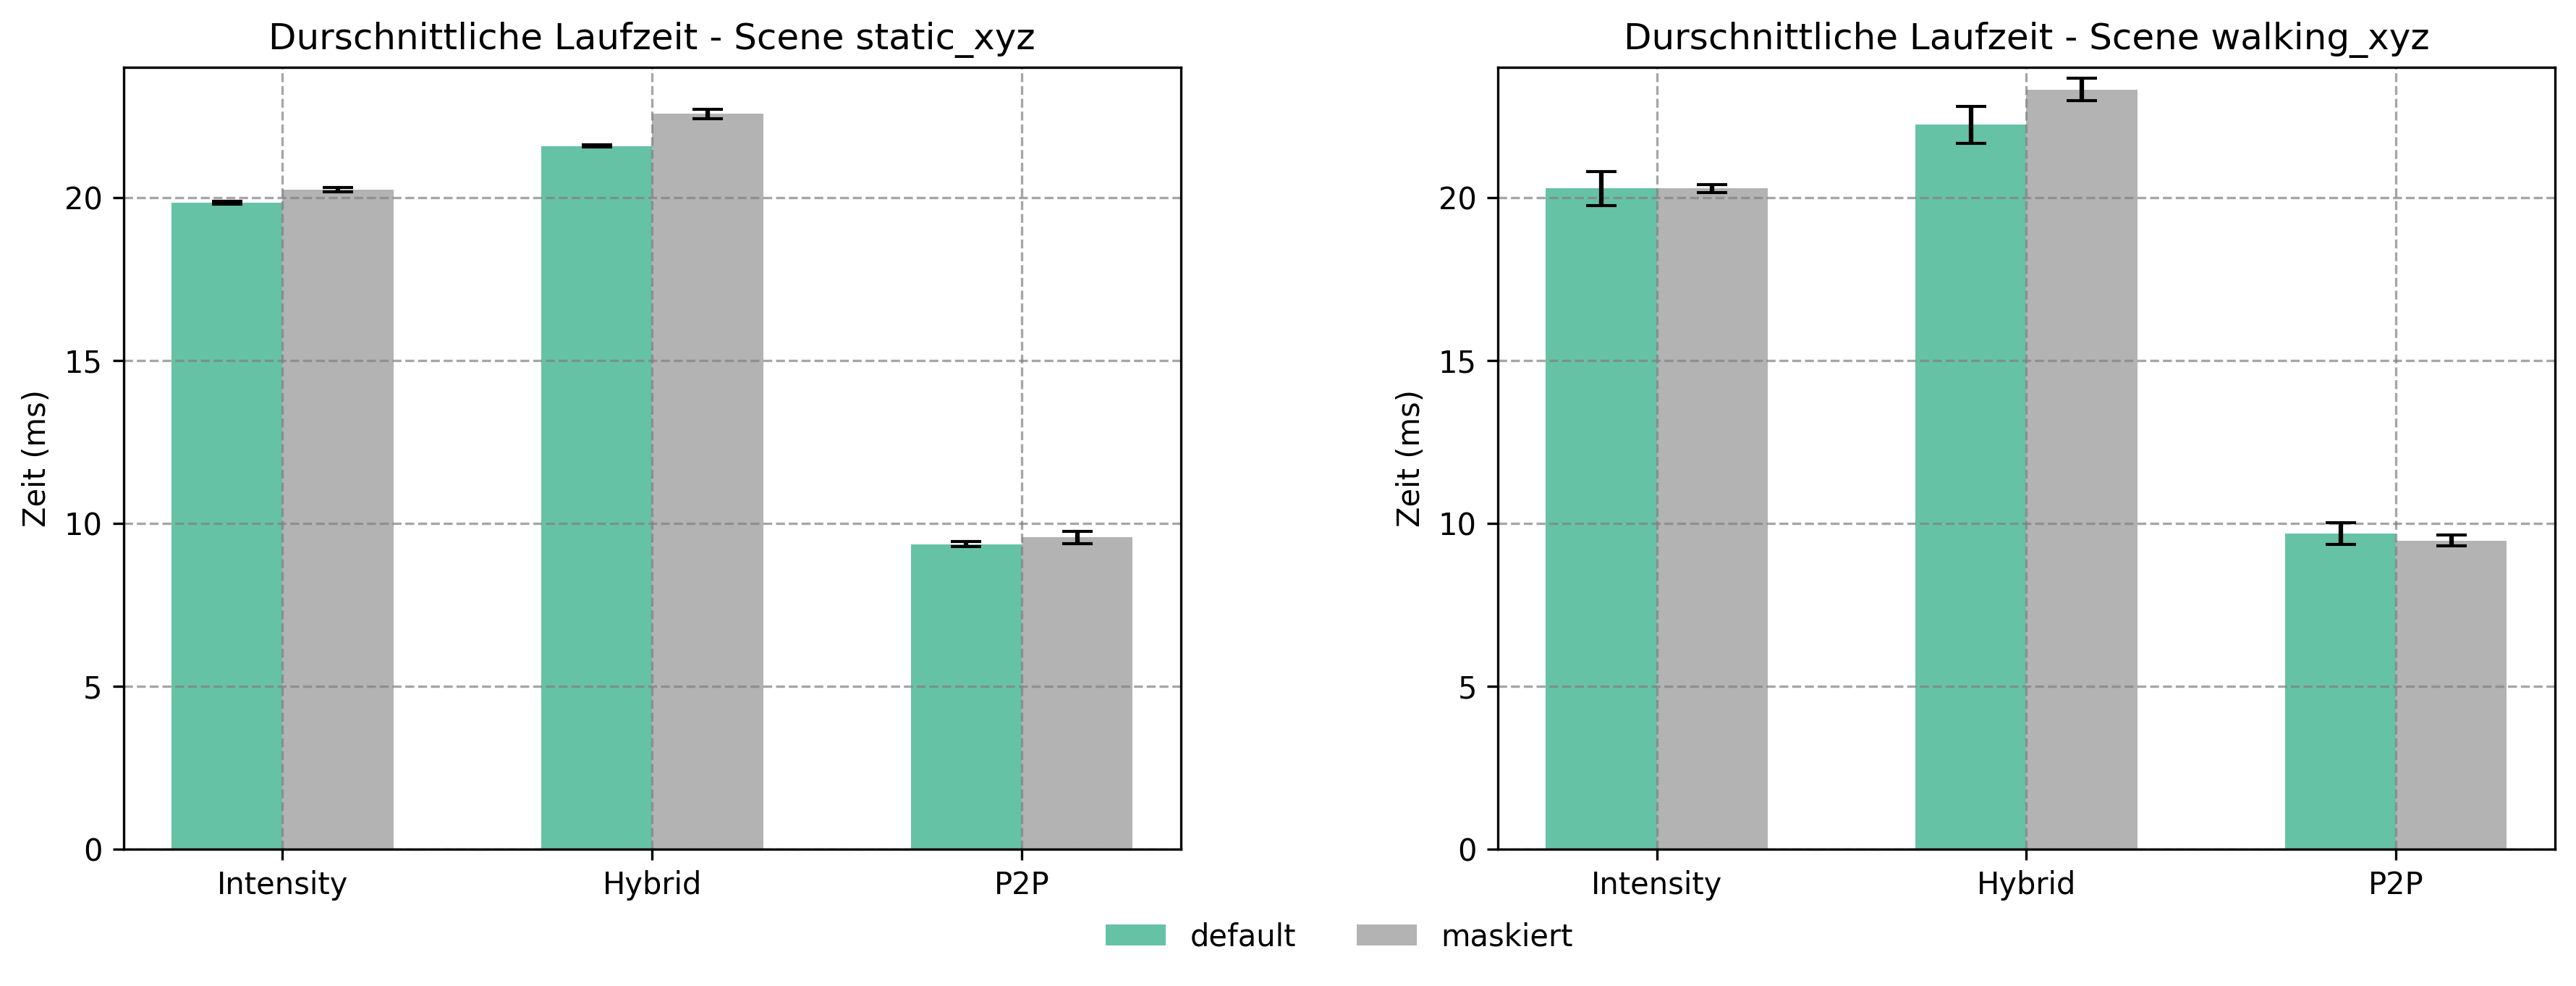
\includegraphics[width=\textwidth]{pics/odom_time_avg.png}
        \caption{durchschnittliche Laufzeit visueller Odometrie. Vergleich von statischer und dynamischer Umgebung durch die Szenen \glqq static xyz \grqq
        und \glqq walking xyz \grqq}
        \label{fig:avg_Laufzeit}
    \end{figure} \noindent
    In der Grafik \ref{fig:avg_Laufzeit} ist zu erkennen, dass jede betrachtete Konfiguration in Echtzeit läuft (für dichtes visuelles Tracking ist eine 
    Framerate von 30 Fps üblich).
    Die Laufzeiten der Intensität's und Hybrid Fehlerfunktion sind deutlich höher als die des \ac{P2P}. Dies kann durch eine erhöhte Belastung des Speicher 
    erklärt werden. Auch ist der Rechenaufwand zum Bestimmen der Gradienten-Bildern über die Sobel-Filter pro Pyramiden-Stufe, ein Faktor.\\\\
    Der Unterschied zwischen der maskierten Variante und der Open3D Implementation ist dagegen kleiner. Das kann mit dem kleineren Speicheraufwand der Masken 
    erklärt werden. Diese werden als 1-Byte pro Pixel Buffer abgespeichert.\\\\
    In den dynamischen Szenen ist ein leichter Trend der Verringerung der 
    Laufzeit in den maskierten Varianten zu erkennen. Ein Entfallen von Jacobimatrix Berechnungen kann ein Grund für das Verhalten liefern.

    \subsubsection{Drift Analyse}
    Visuelle Odometrie bildet einen zentralen Baustein für die Bewegungsbestimmung aus Bilddaten, dabei ist sie jedoch nicht direkt mit einem 
    \ac{vSLAM}-System vergleichbar. 
    In der Tabelle~\ref{tab:ATE_odom_eval} ist eine starke Abweichung der Trajektorie zu erkennen. Für die Bewertung eines solchen Algorithmus ist der \ac{RPE} 
    angebracht.\\\\
    In den Daten \ref{tab:RPE_odom_eval} ist ein klarer Trend erkennbar: Der Translationsfehler des \ac{P2P}-Verfahren weist einen geringeren Drift auf 
    im Vergleich zu den anderen Methoden, unabhängig von der grundlegenden Bewegung. \\\\
    Für den Rotationsdrift zeigt sich ein ähnliches Muster, allerdings weniger ausgeprägt. Die Beobachtung ist nicht als ein Beleg für eine höhere rotatorische 
    Robustheit des \ac{P2P} zu sehen.
    Dafür spricht die Szene mit starker Rotation und ohne dynamische Objekte („static rpy“), in denen das \ac{P2P}-Verfahren deutlich schlechter performt.\\\\
    \begin{figure}[ht]
        \centering
        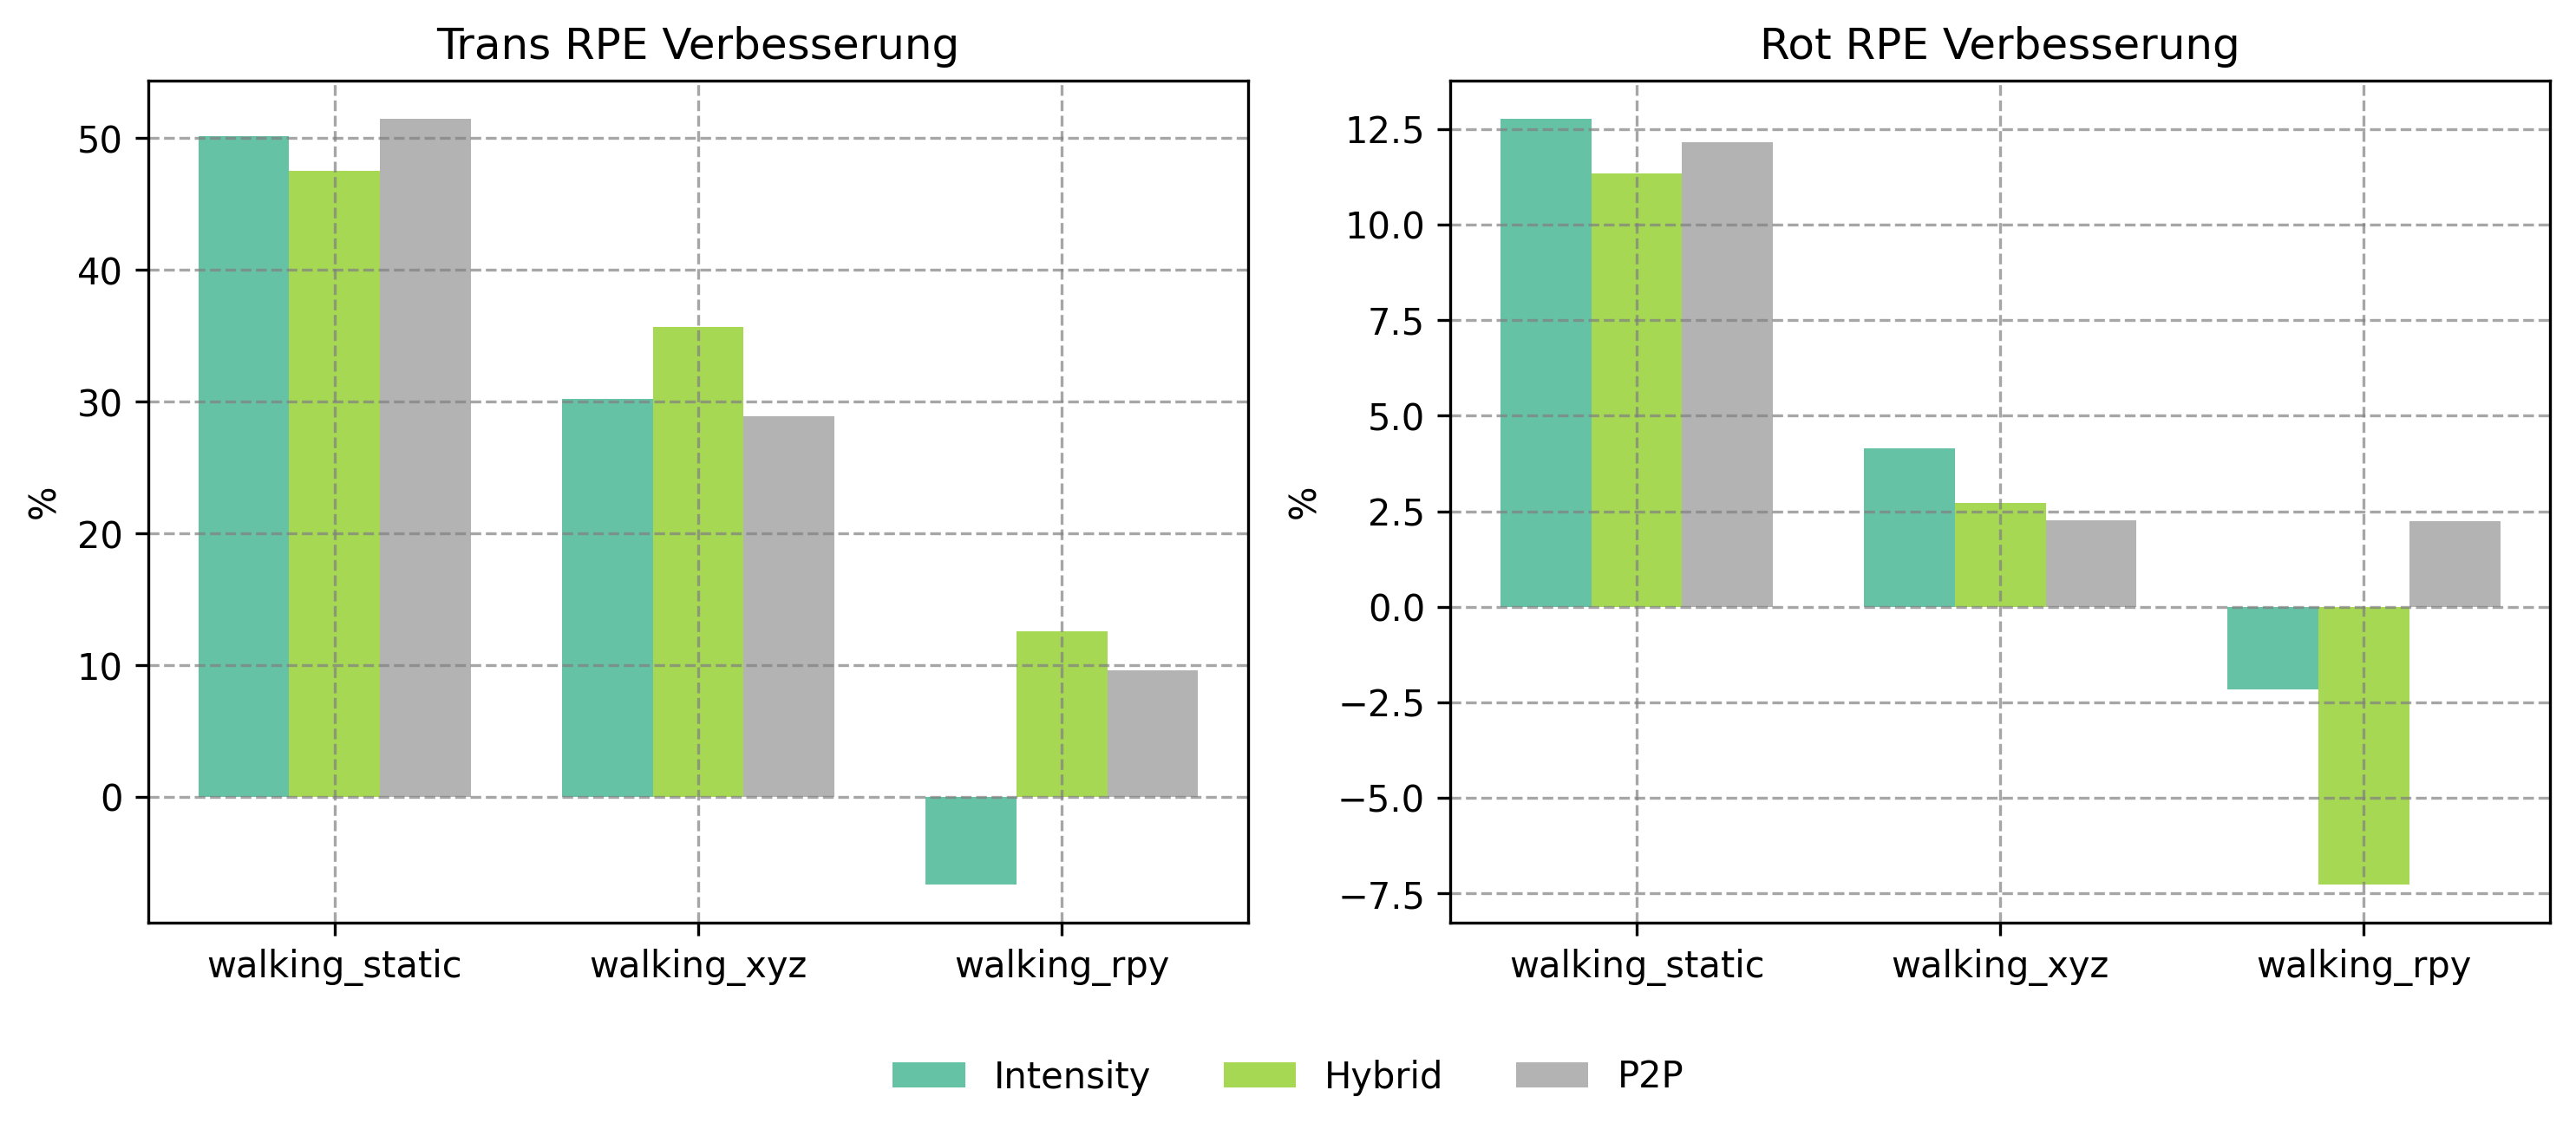
\includegraphics[width=\textwidth]{pics/rel_imp_walking_rpy.png}
        \caption{Prozentuale Verbesserung des RPE durch maskierte Odometrie}
        \label{fig:rel_imp_odom_RPE}
    \end{figure}   
    Auf den statischen Szenen verhalten sich die maskierten Methoden gleich zu den unmaskierten.\\\\
    In den dynamischen Szenen zeigt sich eine deutliche Verbesserung des \ac{RPE} (siehe Abb.~\ref{fig:rel_imp_odom_RPE}). Eine Ausnahme bilden die Rotationsszenen: 
    Hier weist ausschließlich das \ac{P2P}-Verfahren eine Verbesserung auf. \\\\
    Aus den dynamischen Szenen mit unbewegter Kamera lässt sich ableiten, dass das Maskieren eine stabilere Variante des Algorithmus's darstellt.
    Unter dieser Annahme kann das Verhalten in den Rotationsszenen als ein generelles Problem der visuellen Odometrie bei starker Rotation interpretiert werden.
    Unterstützt wird diese Annahme durch den in diesen Szenen erhöhten translationalen Drift.
    
    \subsection{maskiertes TSDF-Tracking Auswertung}
    Der Testaufbau für das \ac{TSDF}-Tracking ist ähnlich zu dem der visuellen Odometrie.
    Dabei wird für die, in dem Algorithmus \ref{alg:tsdf_track} genutzte, visuelle Odometrie die selbe Konfiguration genutzt. Für das Raycasting wird das 
    Standart-Verfahren aus \cite{dong2023ashmodernframeworkparallel,Zhou2018} genutzt. Die Vergleichs-Version des \ac{TSDF}-Tracking in Open3D nutzt zudem auch einen
    Gewichtungswert pro Voxel, um die Stabilität zu erhöhen. Auch in diesem Aufbau wird das Tracking mehrfach auf der gleichen Szene simuliert.
    
    \subsubsection{Laufzeit}
    \begin{figure}[h]
        \centering
        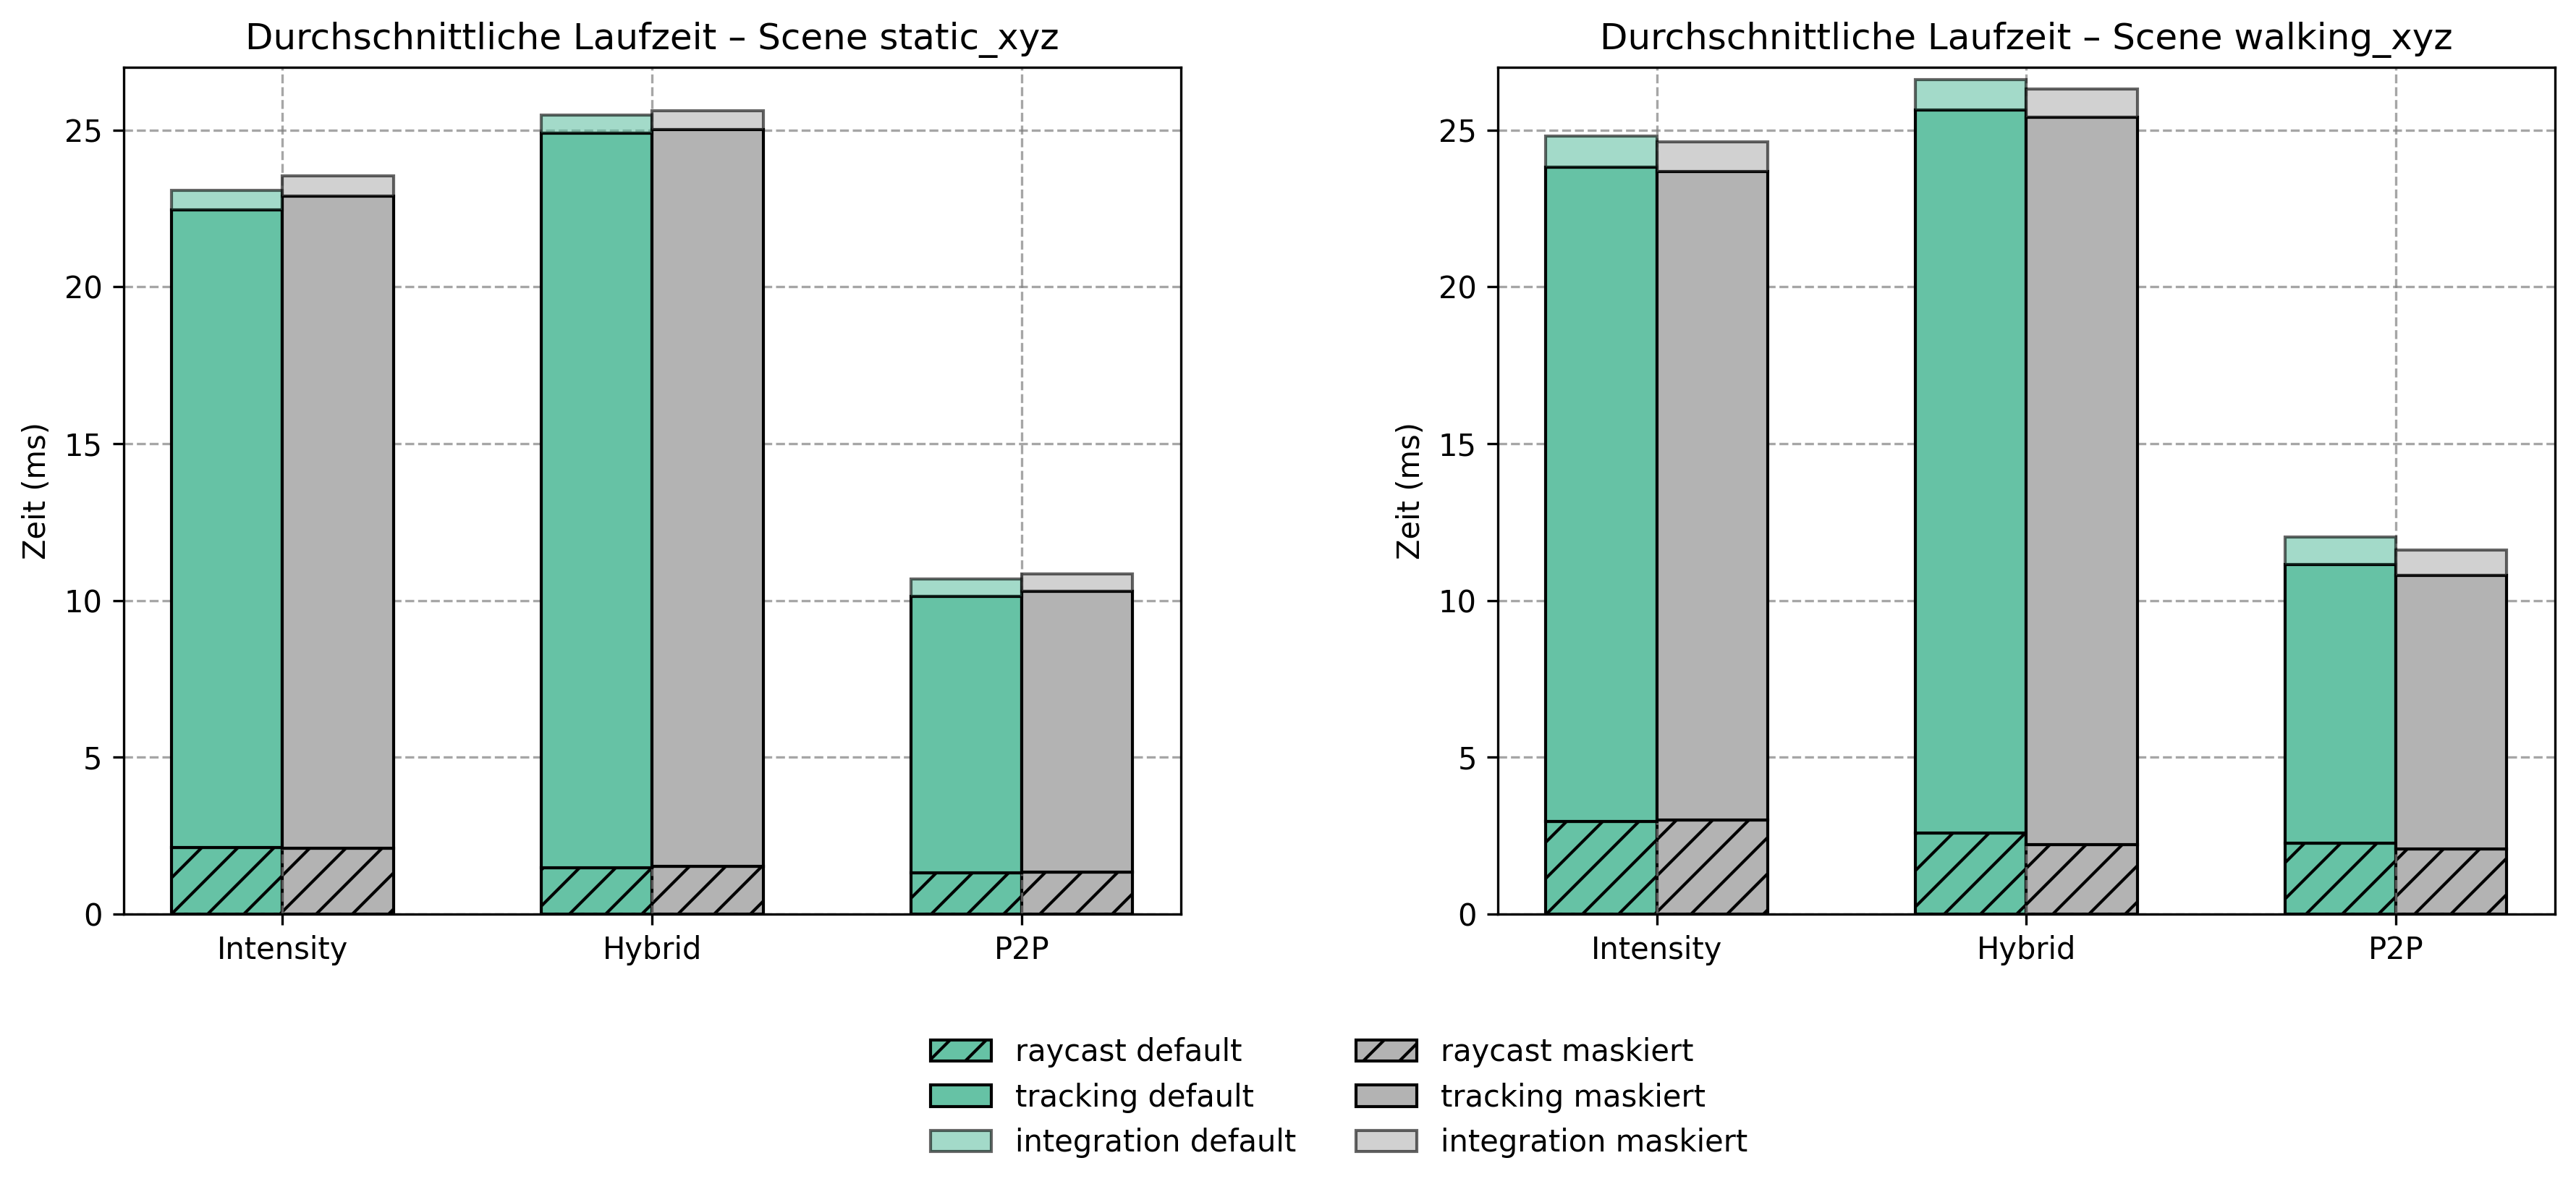
\includegraphics[width=\textwidth]{pics/tsdf_time_avg_split.png}
        \caption{Durchschnittliche Laufzeit des \ac{TSDF}-Trackings. Vergleich von statischer und dynamischer Umgebung durch die Szenen \glqq static xyz \grqq
        und \glqq walking xyz \grqq}
        \label{fig:tsdf_avg_time}
    \end{figure}\noindent
    Ein Großteil der Laufzeit pro Iteration stellt das Tracking durch visuelle Odometrie da (vgl. Abb. \ref{fig:tsdf_avg_time}). Dementsprechend ist das 
    Verhältnis der Laufzeiten für die verschiedenen Fehlerfunktionen vergleichbar zu Abb. \ref{fig:avg_Laufzeit}. \\\\
    Ein weiteres beobachtetes Phänomen ist: Die durchschnittliche Raycasting und Integration Zeit unterscheidet sich zwischen statischer und dynamischer
    Szene. Ein Grund für das Verhalten kann durch die erhöhte Anzahl von aktivierten Blocks und Voxel gefunden werden. In den dynamischen Szenen entsteht
    mehr fehlerhafte Geometrie, die einen negativen Einfluss auf die Rechenzeit des Raycasting und der Integration haben. \\\\

    \subsubsection{Tracking-Verlust}
    In den Daten der Tabellen \ref{tab:RPE_odom_eval} und \ref{tab:RPE_tsdf_eval} ist ein Muster zu beaobachten: Es bestehen starke Schwankungen 
    in \ac{ATE} und \ac{RPE} selbst auf den statischen Szenen. Besonders in den ATE-Werten \ref{tab:ATE_tsdf_eval} sind großen Schwankungen auf gleichen Szene
    zu beobachten.\\\\
    Das ist ein Symptom eines generellen Problem des Trackings mit einem \ac{TSDF}-VoxelBlockGrid, dem Tracking-Verlust. 
    Der Voxel Weighting-Mechanismus, der für die Konsistenz des Modells zuständig ist, kann zu einem Verlust der Referenz von Kamera zu Modell führen.
    Durch schnelle Bewegungen kann es passieren, dass das Kamerasichtfeld auf noch invalide Geometrie gerichtet ist. Dadurch entstehen unvollständige 
    synthetische Bilder. Das Tracking auf Bildern mit einer geringen Anzahl valider Pixel kann zu starken Drift, sowie singulären Gleichungssystemen in der 
    visuellen Odometrie führen.\\\\
    Das Verlieren der Referenz führt dazu, dass die Kameraposition beliebig driftet, bis wieder eine Referenz zu Geometrie gefunden werden kann. Das Ergebnis
    der Rekonstruktion ist dabei Menge von getrackten Fragmenten, in unterschiedlichen Orientierungen und Abständen.\\\\
    Ein Kriterium um einen Tracking-Loss direkt aus den Daten abzulesen, ist eine hohe Varianz in dem \ac{ATE}, durch das nahezu zufällige Driften von Trajektorien.
    \subsubsection{Fehlerfunktionen}
    Anhand der Betrachtung der \ac{ATE}-Varianz ist erkennbar, dass der Intensität's-Fehler anfällig für Tracking-Verlust ist. 
    Die schlechte Performance ist auch erwartbar. Die synthetisch erstellten Bilder simulieren keine n Licht- und Schatten und somit ist ein Vergleich von diesen
    nicht sinnvoll.\\\\
    Ähnliche Probleme sind auch in der Hybrid-Methode zu erkennen. Durch das Einbeziehen der Tiefendaten wird das Tracking verbessert, jedoch tritt auch in 
    der Basis Szenen \glqq static rpy\grqq ein Tracking-Loss auf. Beide Fehlerfunktionen sind somit nicht für das \ac{TSDF}-Tracking geeignet.\\\\
    Die Fehlerfunktion, die von dem Model profitiert, ist die \ac{P2P} Funktion. Die \ac{RPE}- und \ac{ATE}-Werte der statischen Szenen zeigen, dass der \ac{P2P}-Fehler im 
    Vergleich zu den anderen Verlustfunktionen eine stabile und präzise Schätzung liefert. Aus der Abb. \ref{fig:p2p_rel_RPE} ist eine deutlicher Verbesserung des 
    Drifts zu erkennen. Aufgrund der Beobachtung wird im folgenden wird explicit nur der \ac{P2P} genauer in dynamischen Szenen betrachtet.
    \begin{figure}[h]
        \centering
        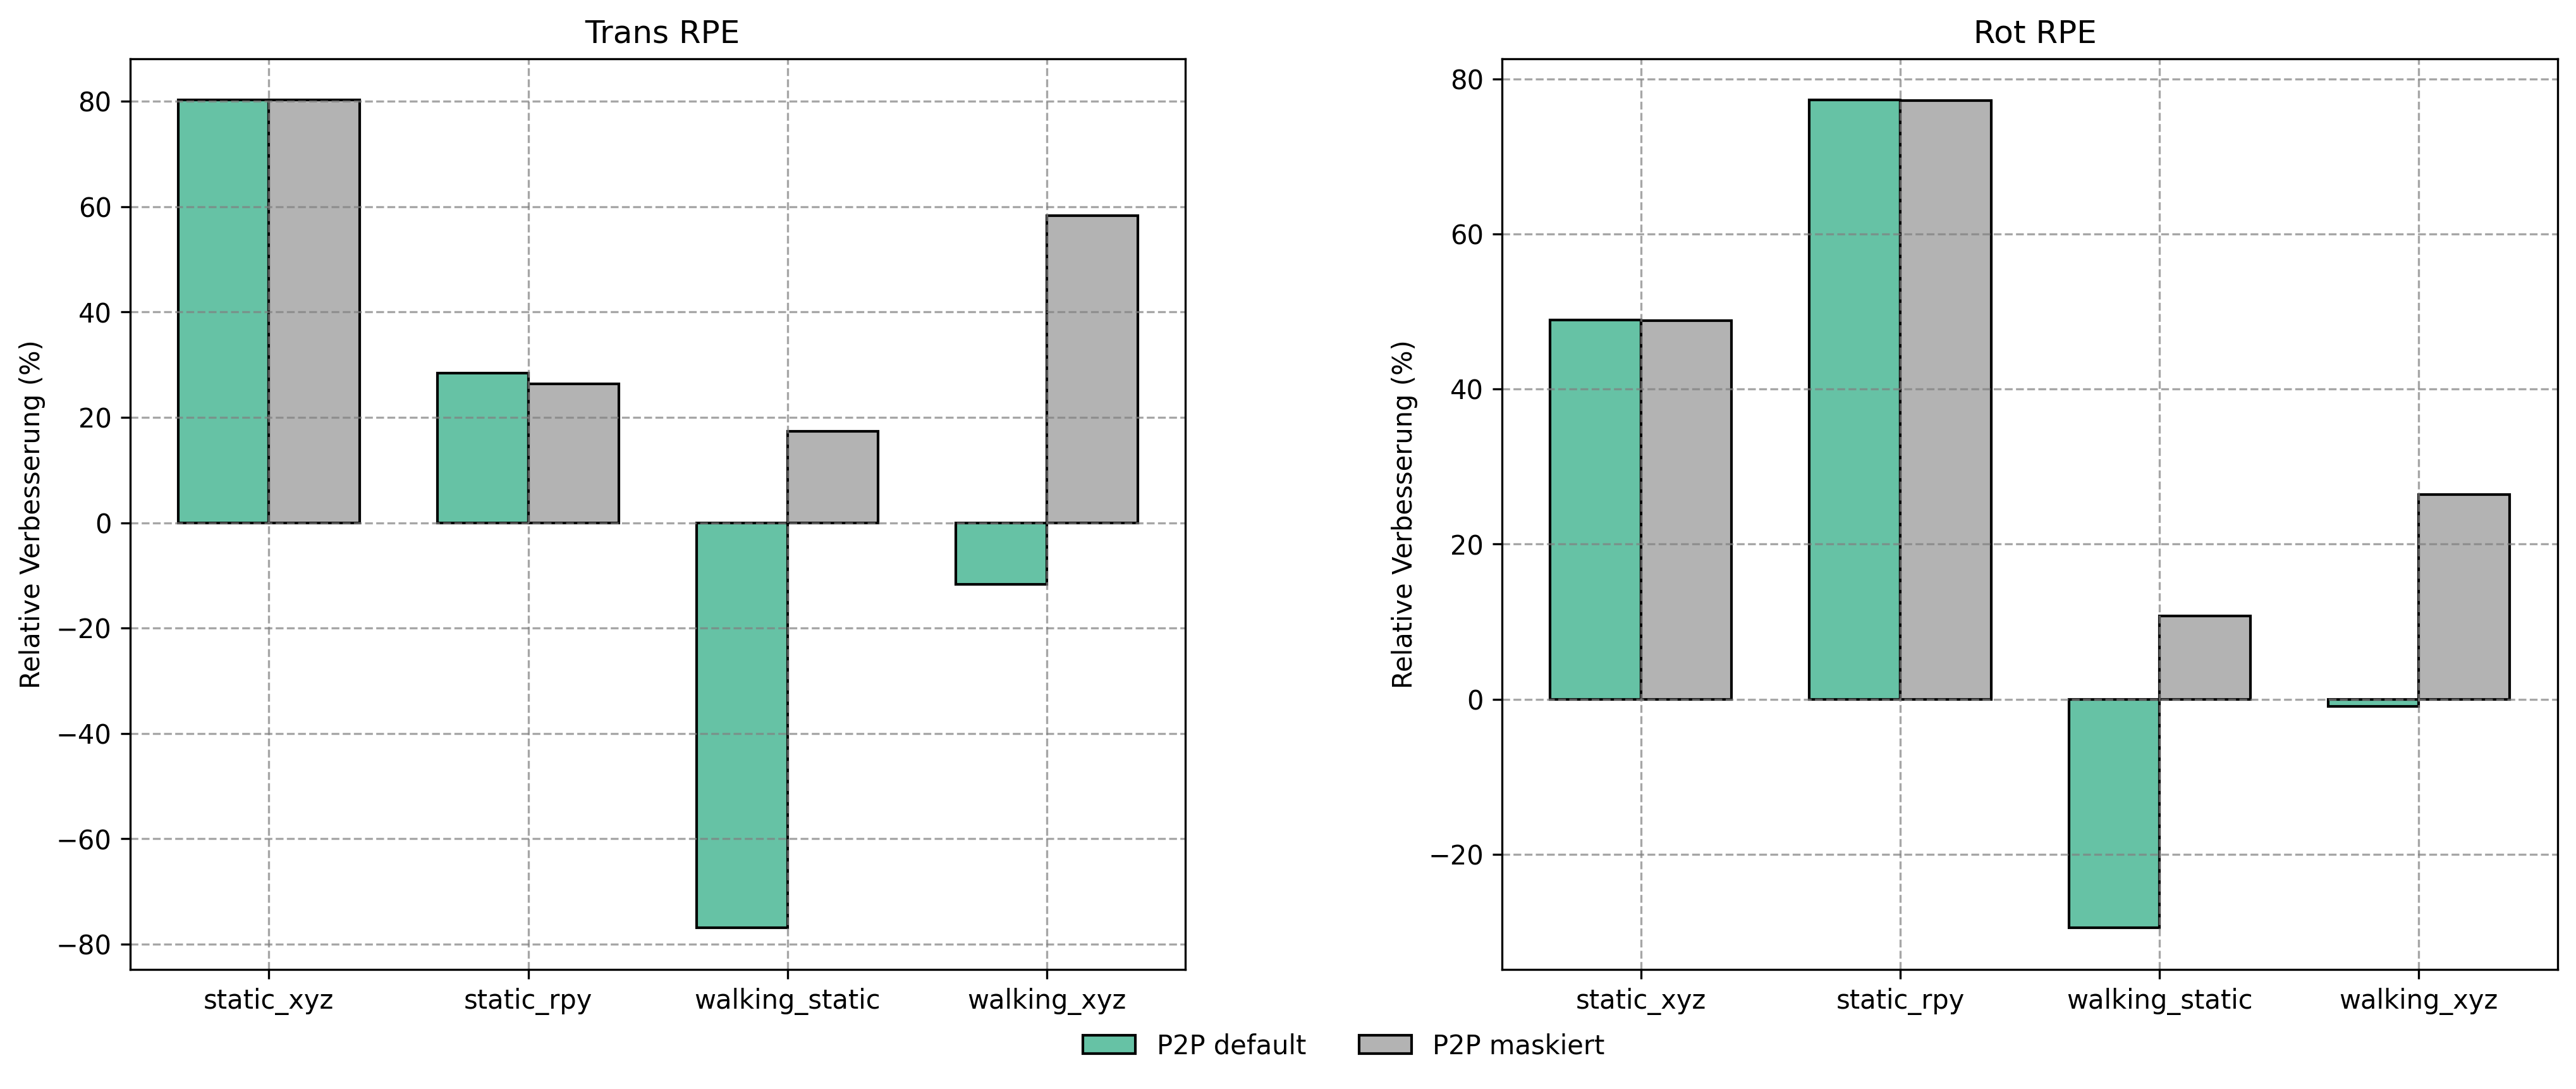
\includegraphics[width=\textwidth]{pics/compose_RPE_com.png}
        \caption{Relative Verbesserung des Drifts der P2P-Fehlerfunktion}
        \label{fig:p2p_rel_RPE}
    \end{figure}

    \subsubsection{dynamische Szenen}
    Die Betrachtung des \glqq Standard\grqq \ac{TSDF}-Tracking auf den dynamischen Szenen zeigt eine Verschlechterung gegenüber der reinen visuellen Odometrie.
    Aus den Varianzwerten des \ac{ATE} auf den dynamischen Szenen ist erkenntlich, dass das \glqq Standard\grqq \ac{TSDF}-Tracking auf jeder das Tracking 
    verliert. Am besten ist dies auf der Szene\glqq walking static\grqq zu erkennen. Trotz keiner Kamera Bewegung entsteht ein Tracking-Verlust. In der Abb. \ref{fig:bild2} ist eine 
    Verschiebung der Szene deutlich zu erkennen.\\\\
    Die Qualität des Trackings ist stark an die der geraycasteten-Bilder gekoppelt. Fehlerhafte Geometrie, die durch bewegende Objekte in das interne 
    Modell eingeführt wird, verschlechtert die Referenzpunkte (vgl. Abb. \ref{fig:bilder_nebeneinander}). Der positive Effekt der synthetischen Bilder ist somit nicht mehr 
    vorhanden und es wird zusätzlich das Tracking behindert.\\\\
    \begin{figure}[ht]
        \centering
        \begin{subfigure}[t]{0.45\textwidth}
            \centering
            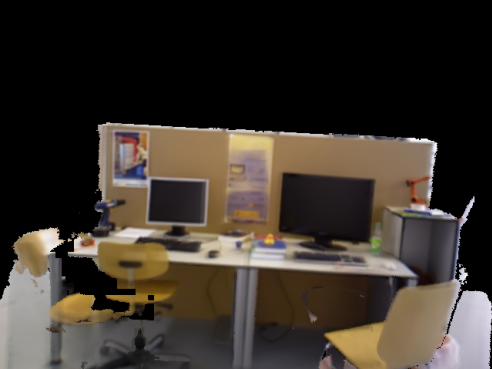
\includegraphics[width=\textwidth]{pics/maskout_image.png}
            \caption{Raycast-Frame maskierte Integration}
            \label{fig:bild1}
        \end{subfigure}
        \hfill
        \begin{subfigure}[t]{0.45\textwidth}
            \centering
            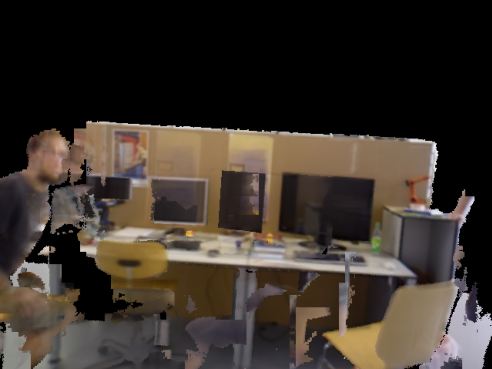
\includegraphics[width=\textwidth]{pics/raw_image.png}
            \caption{Raycast-Frame Open3d standart Integration}
            \label{fig:bild2}
        \end{subfigure}
        \begin{subfigure}[t]{0.45\textwidth}
            \centering
            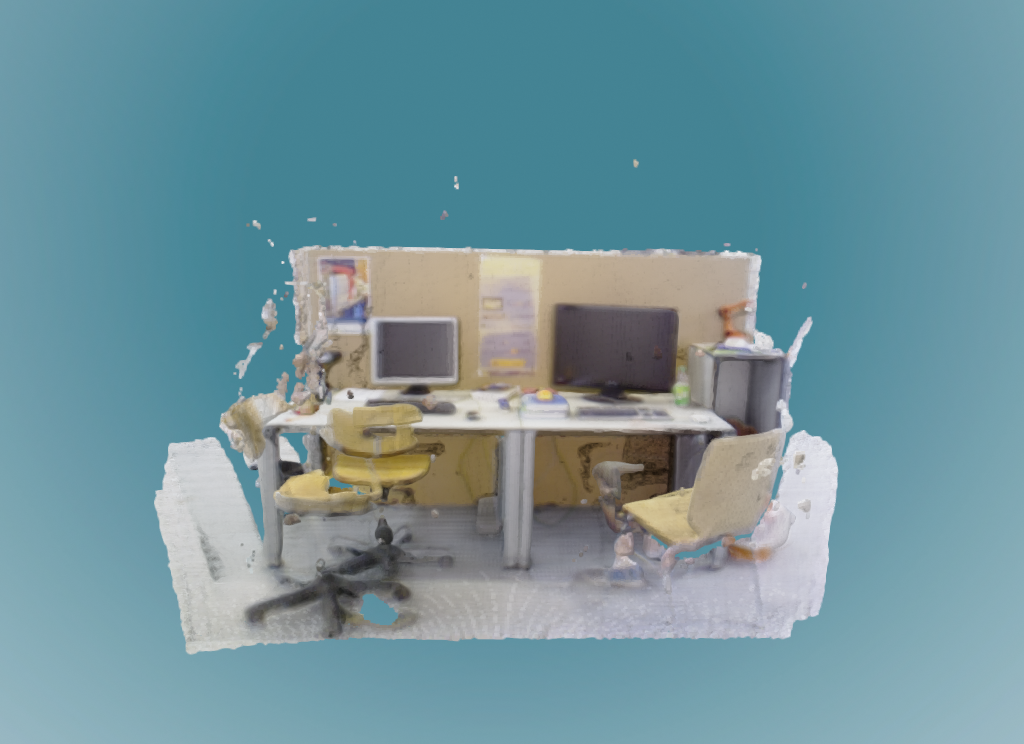
\includegraphics[width=\textwidth]{pics/maskout.png}
            \caption{internes Modell erstellt durch maskierte Integration}
            \label{fig:recon_mask}
        \end{subfigure}
        \hfill
        \begin{subfigure}[t]{0.45\textwidth}
            \centering
            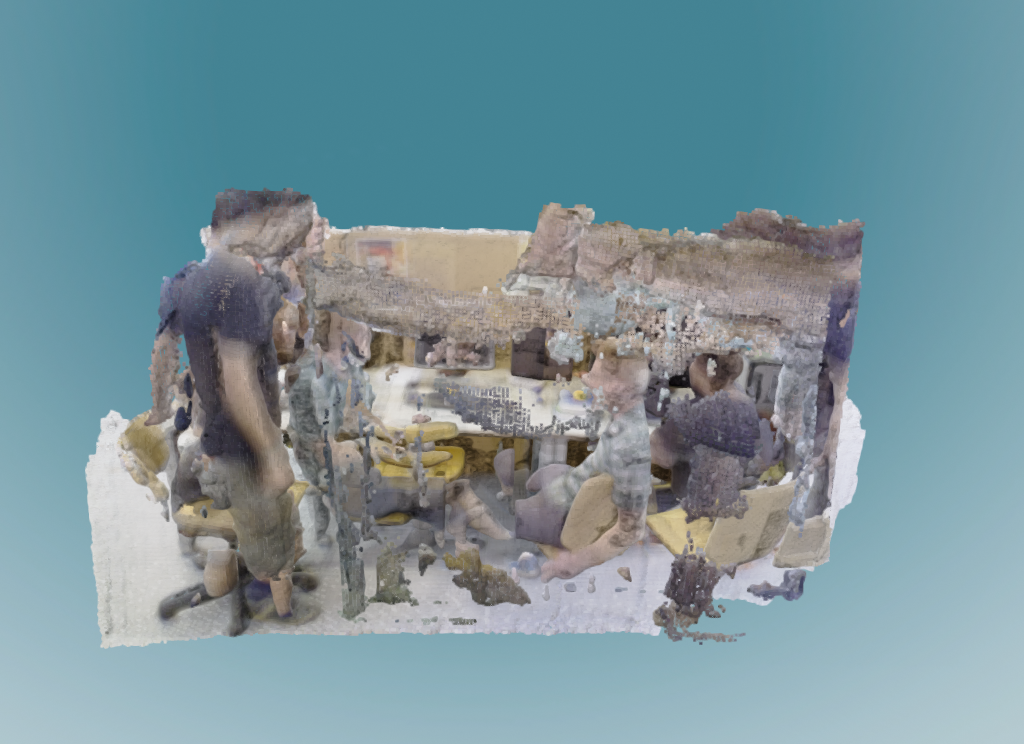
\includegraphics[width=\textwidth]{pics/raw.png}
            \caption{internes Modell erstellt durch Open3d standart Integration}
            \label{fig:recon_raw}
        \end{subfigure}
        \caption{Integrations Algorithmen Vergleich}
        \label{fig:bilder_nebeneinander}
    \end{figure}
    Der maskierten Variante des \ac{P2P} \ac{TSDF}-Trackings, ist es als einzigen Konfiguration möglich auf den dynamischen Szene ein Tracking-Loss zu vermeiden. 
    Dabei steht die dynamische Rotations-Szene hervor. Die Verbindung aus Rotation und bewegter Szene erschwert das Tracken immens.
    Wie schon in Section \ref{sec:aus_vis_odom} betrachtet besitzt der visuelle Odometrie Algorithmus Schwierigkeiten auf der Rotations-Szene.

    \subsection{Bewertung}
    Die beschrieben Experimente zeigen deutlich, dass der \ac{P2P} den Intensität's und Hybrid Fehler überlegen ist. Ähnliche Beobachtung wurden auch in 
    \cite{rusinkiewicz2001efficient} getätigt.
    In der Laufzeit ist die \ac{P2P} Fehlerfunktion auch deutlich überlegen. 
    Das Muster setzt sich auch auf das \ac{TSDF}-Tracking fort. Dieser Trend ist jedoch erwartbar, da die synthetischen Bilder das Tracking per Intensität's Werten 
    behindert.\\\\
    Die  maskierten Varianten der Methoden stellen eine Verbesserung in den einzelnen Algorithmen da. Besonders ist dieser Trend bei dem \ac{TSDF}-Tracking
    zu erkennen. Es ermöglicht erst eine Fortsetzung des Verfahrens auf dynamische Szenen.\\\\
    Die Ergebnisse zeigen jedoch auch, dass weder die visuelle maskierte Odometrie noch das \ac{TSDF}-Tracking ein zuverlässiges und robustes Tracking gewährleisten.
    Wie in Tabelle~\ref{tab:ATE_odom_eval} ersichtlich, ist die reine Odometrie stark fehleranfällig.
    Das maskierte \ac{TSDF}-Tracking mit der \ac{P2P}-Fehlerfunktion bietet eine deutliche Verbesserung, leidet jedoch unter hoher Instabilität:
    Bei langsamer Bewegung und geringer Rotation arbeitet es zuverlässig, während stark dynamische Bewegungen zu einem vollständigen Trackingausfall führen.\\\\ 
    Somit stellen beide Verfahren kein robustes \ac{vSLAM}-System dar.
    Sie können jedoch als Komponenten in einem System eingesetzt werden, das mehrere Tracking-Algorithmen kombiniert und deren Ergebnisse fusioniert.
    Ein solches Zusammenspiel unterschiedlicher Verfahren mit jeweils eigenen Stärken und Schwächen ist charakteristisch für leistungsfähige \ac{SLAM}-Systeme.\\\\
    Ein möglicher Ansatz wäre das Tracking durch die visuell basierenden Fehlerfunkionen zu überwachen, um einen möglichen Trackingverlust zu erkennen.
    Das führt jedoch in das diverse und umfangreiche Feld der vSLAM-Systeme, welches nicht genauer betrachtet werden.\\\\
    Für den Einsatz im Stahlumfeld ist das \ac{TSDF}-Tracking trotz der genannten Einschränkungen geeignet. Der Roboter, auf dem das System montiert ist bewegt 
    sich mit einer transitiven Bewegung. Auch ist die Geschwindigkeit des Roboters gering. Somit treten die Hauptkomponenten für eine Tracking-Verlust 
    nicht auf. Die Tiere stellen dabei ein teilweise kontrollierbaren Faktor dar, welchem mit dem maskierten Tracking entgegenwirkt werden kann.

    \chapter{Semantische Bild Segmentierung}\label{sec:SemSeg}
    In dem Gebiet des \ac{vSLAM} sind Deep Learning Methoden essenziell für das Tracking in dynamischen Umgebungen. Dabei sind Bild-Segmentierungs Netzwerke ein 
    wichtiger Bestandteil. Speziell bei der Rekonstruktion der Futterstelle sind Masken, als Eingabe in die maskierten Algorithmen nötig (siehe \ref{kap:maskout}).\\\\
    Bei der Bildsegmentierung wird unterschieden zwischen der \ac{GIS} und \ac{PIS}. Während \ac{PIS} speziell für promptfähige Modelle entwickelt ist, die 
    ihre Segmentierung auf textuellen oder exemplarischen Eingaben basieren, beschreibt \ac{GIS} das automatische Klassensegmentieren ohne zusätzliche 
    Benutzereingaben (vgl. \cite{zhou2024imagesegmentationfoundationmodel}). Das automatische Generieren von Kuh-Masken fällt in das Gebiet des \ac{GIS}.
    Grundlegende  Problemstellungen des \ac{GIS} sind (vgl. \cite{zhou2024imagesegmentationfoundationmodel, csurka2023semanticimagesegmentationdecades}):
    \begin{itemize}
        \item \textbf{Semantische Segmentierung:} Jeder Pixel in einem Bild wird ein Klassenlabel zugeteilt
        \item \textbf{Instanzen Segmentierung:} Pixel werden in zusammenhängende Regionen gruppiert
        \item \textbf{Panoptic Segmentation:} Verbindung Instanzen und semantischer Segmentierung
    \end{itemize}
   

    \section{Datensatz}
    Der Datensatz besteht aus einer Menge an Kamerafahrten, die in dem selben Stall aufgenommen wurden. Dabei wird in jeder Videoaufnahme eine Fahrt des 
    Schieberoboters simuliert. Sie unterscheiden sich untereinander in der Orientierung des Sensors zu der Futterstelle und in dem Sichtfeld.\\\\
    Die Aufnahmen stellen hoch dynamische Szenen da, mit vielen, sich im Hintergrund und Vordergrund, bewegenden Kühen. Viele Kühe sind dabei verdeckt oder 
    klein im Hintergrund sichtbar. Die Lichtverhältnisse variieren, wodurch die Qualität der Bilder gemindert wird.
    Insgesamt besteht der Datensatz aus 6 Kamera-Läufen und insgesamt 350 Bildern. Die Auflösung der Bilder in dem Datensatz ist 640x480.\\\\ 
    Die in dem Datensatz annotierten Klassen sind:
    \begin{itemize}
        \item \textbf{Kühe:} Für das Maskieren in den Tracking und Rekonstruktion-Algorithmen
        \item \textbf{Silage:} Als Grundlage in der Futtermessung
        \item \textbf{Background:} Die restliche Szene
    \end{itemize}\noindent
    Durch Unterschiede in der Kamera-Positionierung besteht in bestimmten Kamerafahrten eine starke Klassen-Ungleichheit. Dabei stellt der Hintergrund und die Silage
    einen Großteil der Pixel da. In anderen Kamerafahrten dominieren die Kühe als Klasse die Bilder.

    \subsection{Annotation}
    Die Annotation stellt einen aufwendigen Teil in der Erstellung des Datensatzes da. Für die semantische Segmentierung muss eine Klassifikation pro Pixel annotiert 
    werden. Um den Prozess zu erleichtern ist die Nutzung von existierende Segmentierungs-Modellen im Labeling Prozess essenziell.\\\\
    Die unmittelbare Nutzung von \ac{GIS} Segmentierungsmodell ist nicht möglich. Aufgrund der Komplexität der gefilmten Szene,
    sowohl als auch der spezifischen Anforderungen der Klassen, ist viel manuelles Postprocessing für die Masken nötig.\\\\
    Für effektiveres und interaktives Labeln können \ac{PIS} Segmentierungs-Modells genutzt werden. Konkret wurde das SAM2 \cite{ravi2024sam2segmentimages} 
    verwendet. Das Modell 
    bietet die Möglichkeit Segmentierung aufgrund von visuellen Promts zu erreichen. Dafür können Punkte, Bounding-Boxes und Vorsegmentierung als Input in 
    das Modell gegeben werden. Somit ist ein flexibles und schnelles Segmentieren von selbst schwer semantisch zu erkennenden Regionen möglich.
    Trotz dem flexiblen Labeling Setup ist manuelles Postprocessing nötig.\\\\
    Die Segmentierungen sind nicht pixelgenau. Aufgrund ungünstiger Lichtverhältnisse lassen sind Kühe im Hintergrund schwer oder gar nicht erkennen. Teile
    der Bilder stellen nicht erkennbare Regionen da, in denen eine Annotation nicht möglich ist.

    \subsection{Evaluation und Trainingsdatensatz}

    Der Datensatz weist Herausforderungen auf. Bilder aus demselben Durchlauf sind aufgrund temporaler Überschneidungen stark miteinander korreliert.
    Daher ist bei der Trennung in Trainings- und Validationsdaten besondere Vorsicht geboten.
    Ein akkurates Vorgehen wäre, für Trainings- und Validationsdatensatz Aufnahme aus verschiedenen Ställen zu verwenden. Das ist jedoch zu diesem
    Zeitpunkt nicht möglich. Zukünftig ist geplant, den Datensatz in dieser Hinsicht zu diversifizieren.\\\\
    Eine perfekte Trennung der Daten ohne Korrelation zwischen Splits ist nicht möglich. Der Hintergrund, sowie die Futterstelle bleiben unverändert 
    zwischen Aufnahmen. Das bestmögliche Vorgehen auf dem Datensatzin in seinem derzeitigen Zustand ist eine Trennung anhand der einzelnen Kamerafahrten.\\\\
    Aufgrund einer Imbalance zwischen der Anzahl der Bilder in den einzelnen Läufen bringt das Vorgehen Probleme mit sich.
    Eine faire Trennung ist nicht ohne große Variation der Große von Validationsdatensatze oder einem großen Verlust von annotierten Bilder möglich.\\\\
    Die gewählte Trennung besteht aus einer Unterteilung in den einzelnen Kamerafahrten. Damit die Trainings- und
    Evaluationsdatensatz nicht stark korrelieren werden zeitliche Pufferzonen eingebaut. Die Lösung ist nicht optimal, da starke Zusammenhänge 
    zwischen Splits fortbestehen.\\\\
    Die Wahl der Splits beeinflusst die zeitliche Position der Validations-Bilder. Um diesen Faktor zu kontrollieren wird
    ein Teilung mithilfe von 5-Folds Crossvalidation festgelegt. Dabei werden die temporalen Abschnitte zufällig in jeder Fahrt gewählt, ohne dass dabei
    einen eine Menge von Bildern mehrfach als Validationsdatensatz vorkommt.\\\\
    Dieses Vorgehen ist nicht akzeptabel für einen Testdatensatz. Daher stellt dieser eine eigenen Kamerafahrt da. 
    Ein großes Problem ist: Die Test-Aufnahme stammt von dem selben Tag und Stall. Es bestehen somit strake Korrelation, was die Genrealisierbarkeit der 
    erzielten Ergebnisse deutlich infrage stellt.

    \subsection{Augmentation}
    Aufgrund der kleinen Große des Datensatzes werden die Bilder im Training konstant augmentiert. Dafür wird eine zufällige Spiegelung und eine zufällige
    Verkleinerung um 20 \% des Bildbereiches auf ein Bild angewendet .  
    Solche augmentation stellen ein Stadtartvorgehen in der Bildsegmentierung da (vlg. \cite{chen2017rethinkingatrousconvolutionsemantic,HaitzHuebnerUlrich2022}).

    \section{Model-Architektur}
    Für die semantischen Segmentierung von Bildaufnahmen existieren zahlreiche Ansätze. Eine weit verbreitete Herangehensweise basiert auf 
    überwachtem Lernen, wobei insbesondere Architekturen auf Grundlage von \ac{CNN}'s häufig eingesetzt werden. Darüber hinaus wurden verschiedene Erweiterungen 
    entwickelt, die beispielsweise Attention-Mechanismen, Conditional Random Fields oder Recurrent Neural Networks einbeziehen. In jüngerer 
    Zeit haben zudem Transformer-Modelle zunehmend an Bedeutung gewonnen (vgl. \cite{csurka2023semanticimagesegmentationdecades,
    zhou2024imagesegmentationfoundationmodel, minaee2020imagesegmentationusingdeep}).\\\\
    Als Architektur wird DeepLabV3+  \cite{chen2018encoderdecoderatrousseparableconvolution} gewählt, eine aktuelle Weiterentwicklung der DeepLab-Familie. Diese Modelle basieren auf dem Konzept der 
    Atrous Convolutions und integrieren moderne Erweiterungen wie Encoder-Decoder-Strukturen
    \cite{chen2018encoderdecoderatrousseparableconvolution,chen2017rethinkingatrousconvolutionsemantic}. 
    DeepLabV3+ stellt eine weit verbreitete Architektur dar, die sowohl in der Forschung als auch in 
    zahlreichen industriellen Anwendungen erfolgreich eingesetzt wird (vgl. \cite{csurka2023semanticimagesegmentationdecades, 
    minaee2020imagesegmentationusingdeep}). Die Grundlage von Deeplab bildet ein abgepasstes \ac{FCN}. \\\\
    \subsection{CNN-Backbone}
    Um die Deeplab Architektur zu verstehen muss zuerst die Funktionsweise von \ac{FCN}'s verstanden werden.  
    \ac{FCN} basieren auf der Convolution (Faltung) als zentrale Operation. 
    \begin{defi}
    Sei $\Omega := \{0, \ldots , W-1\} \times \{ 0, \ldots, H-1\} \times  \{ 0, \ldots,C_{in}\}$, dann wird ein Bild (Feature Map), mit Auflösung $H\times W$ 
    und $C_{in}$ Featurechannels, definiert durch $I: \Omega \to \mathbb{R}$.\\\\
    Weiter sei $\Omega^* := \{0, \ldots , k_w\} \times \{ 0, \ldots, k_h\} \times \{0, \ldots, C_{in} \} \times  \{0, \ldots,C_{out}\} $. Dann ist ein 
    Convolution Kernel (Faltungskerne) mit Kernel Größe $k_w  \times k_h$ für $C_{in}$ Input Feature Channels Feature Channels und $C_{out}$ Output 
    Channels gegeben durch $K: \Omega^* \to \mathbb{R}$.\\\\
    Eine $k_w\times k_h$ Bildfaltung (Image-Convolution) zu dem Kernel K, ist definiert als:  
    \[
    (I * K)(x, y, c) = \sum_{i =0}^{k_h-1}\sum_{j=0}^{k_w-1} \sum_{d = 0}^{C_{in}-1}I(x-i +a, y-j+b, d)K(i,j,d,c)
    \]
    Dabei sind $a = \lfloor \frac{k_w}{2} \rfloor, b = \lfloor \frac{k_h}{2} \rfloor$. Eine Convolution mit $K$ erzeugt ein neues Bild $I * K$ 
    mit $C_{out}$ Feature Channels.\cite{pytorch_Convolution}
    \end{defi} \noindent
    Die Faltung mit einem Kern $K$ stellt eine gewichtet Summe über die Input-Feature Channels eines lokalen Fenster's der Große $k_w \times k_h$ dar. 
    Durch den Kern $K$ werden $C_{out}$ viele Gewichtungen separat durchgeführt.\\\\
    Einzelne Convolution-Schichten in einem \ac{FCN} bestehen jeweils aus einem zu lernenden Kern $K$. Das allgemeine Prinzip besteht darin, die Anzahl der 
    Feature-Channels sukzessive zu erhöhen, indem Faltungen mit zunehmender Ausgabedimension $C_{out}$ angewendet werden. Eine kontinuierliche Erhöhung der 
    Kanalanzahl ist jedoch nicht praktikabel, da der Speicherbedarf bei hochaufgelösten Feature-Maps stark ansteigt.\\\\
    Aus diesem Grund wird die Kanalanzahl typischerweise nur bei gleichzeitiger Verringerung der räumlichen Auflösung der Feature-Maps erhöht. Eine Methode 
    für das Verkleiner'n der Auflösung sind strided Convolutions.
    \begin{defi}
    Sei I ein Feature-Map und $K$ ein Faltungskern. Weiter seien $s_h, s_w \in \mathbb{N}$, dann ist die 
    strided Bildfaltung zu dem Kernel K definiert durch 
    \[
    (I * k)(i, j, c) = \sum_{i =0}^{k_h-1}\sum_{j=0}^{k_w-1} \sum_{d = 0}^{C_{in}-1}I(x *s_h-i +a, y*s_w-j+b, d)K_{i,j,d,c}
    \]
    \end{defi}\noindent
    Die Werte $s_h, s_w$ stellen die Schrittweiten der Mittelpunkte des Kernelfenster da. Mit geschickter Wahl von Padding und Schrittweiten wird 
    die Auflösung halbiert und gleichzeitig die Anzahl der Feature Channels verdoppelt. Der Faktor um den Auflösung reduziert 
    wird, wird als der Outputstride bezeichnet. Eine Outputstride von 32 und größer ist geläufig. 
    \begin{remark}
    In \ac{FCN} werden neben strided Convolutions auch Pooling Layers genutzt um die Auflösung zu verkleinern. Bei einem Pooling-Layer wird auf Fenstern
    Durchschnitt's Werte oder Maxima berechnet der Channels berechnet.
    \end{remark}

    \subsection{Encoder}
    Der Encoder von Deeplab besteht großteils aus dem Backbone Model. Dieses liegt in modifizierter Form vor. 
    Das Problem welches auftritt, wenn das unveränderte Backbone Model genutzt wird ist, dass der Outputstride groß ist. Um auf die originale Auflösung 
    zukommen müssen die  Features dementsprechend hochskaliert werden, was zu einer groben Akkuratheit der Pixel Klassifikation führt. 
    Das Vorgehen besteht darin, den Outputstride des Backbone-Modells niedrig zu halten.
    \subsubsection{Atrous Convolutions}
    Ein niedriger Outputstride führt zu unerwünschten Folgen. Convolutions in späteren Schichten haben die die Eigenschaft, dass durch die Verringerung
    der Auflösung, größere Bildbereiche durch Convolution-Fenster wahrgenommen werden. Um das Verhalten zu emulieren werden sogenannte Atrous Convolutions genutzt. 
    \begin{defi}
    Sei I ein Bild und $K$ ein Faltungskern. Weiter seien $r_h, r_w \in \mathbb{N}$, dann ist die 
    Atrous Bildfaltung zu dem Kernel K definiert durch 
    \[
    (I * k)(i, j, c) = \sum_{i =0}^{k_h-1}\sum_{j=0}^{k_w-1} \sum_{d = 0}^{C_{in}-1}I(x-i*r_h +a, y-j*r_w+b, d)K(i,j,d,c)
    \]
    \end{defi}\noindent
    Atrous Convolutions simulieren eine Ausbreitung des Faltungsfensters. Ab einem festen Outputstride werden strided Convolution durch 
    entsprechenden Atrous Convolution ersetzt \cite{chen2017rethinkingatrousconvolutionsemantic}.
    \begin{remark}
    \label{bem:backboneparam}
        In der Implementation werden vortrainierte Parameter von dem Backbone Model genutzt werden (vgl. \cite{chen2017rethinkingatrousconvolutionsemantic,HaitzHuebnerUlrich2022}). 
        Da die Anzahl der In- und Output-Channels unverändert bleibt, 
        sowie die Dimension der Kernelfenster, stimmen die Dimension für die Parameter überein. Auch bleibt der Sichtbereich der Fenster durch die 
        Ausbreitung gleich, was eine Rechtfertigung für die Sinnhaftigkeit der Parameter des Backbone-Models gibt.\\\\
        Wichtig dabei ist anzumerken, dass aufgrund der höheren Auflösung der Speicherplatz der Feature Maps ansteigt, sowie der Rechenaufwand, da die Fenster auf 
        mehr Pixel operieren . \cite{Deeplabv3plus_PyTorch}
    \end{remark}

    \subsubsection{Astrous Spatial Pyramid Pooling}
    Eine Innovation die spätere Deeplab-Architekturen anwenden, ist das \ac{ASPP}. Ein generelles Vorgehen in Segmentierungs-Modellen sind
    Bild-Pyramiden Module. Sie sollen die Intrinsische Lokalität von Convolution entgegen wirken, indem mehren Bildskalen gleichzeitig betrachtet werden
    (vlg. \cite{csurka2023semanticimagesegmentationdecades}). 
    Deeplab nutzt dabei Atrous-Convolutions um Multiskalen-Daten zu erfassen \cite{chen2017rethinkingatrousconvolutionsemantic}. Dafür werden
    mehrere separable Atrous Convolution mit unterschiedlichen Raten und Padding in parallel auf eine Feature Map angewandt (siehe \ref{fig:deeplabv3plus}). 
    Zudem wird eine 1x1 Convolution und ein 2x2 Average Pooling Layer genutzt. \\\\
    Das Padding in den Atrous Convolution wird dabei so gewählt, dass die Auflösung der Feature Map erhalten bleibt.
    Der Output des Pooling Layers wird auf die dieselbe Auflösung hoch interpoliert. Somit haben alle Outputs 
    die gleiche Auflösung und können verkettet werden. Durch eine $1\times 1$ Convolution werden die Multiskalen Feature-Channel
    kombiniert und projiziert \cite{chen2017rethinkingatrousconvolutionsemantic}

    \begin{figure}[ht]
        \centering
        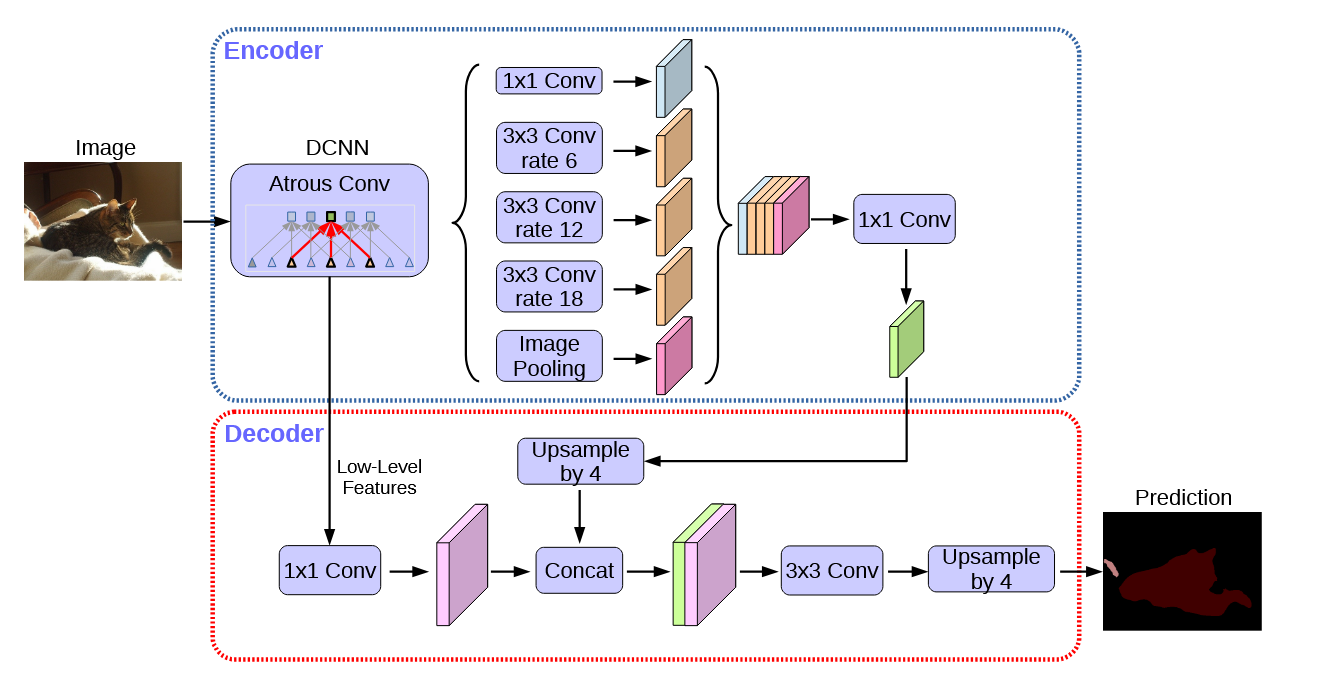
\includegraphics[width=0.9\linewidth]{pics/Arc.png}
        \caption{DeepLabv3+ Architecture (Original aus \cite{chen2018encoderdecoderatrousseparableconvolution})}
        \label{fig:deeplabv3plus}
    \end{figure}

    \subsection{Decoder} 

    In früheren Deeplab Modellen wurden die Ergebnisse des \ac{ASPP} Modules Bilinear auf die originale
    Auflösung hoch interpoliert. Eine Verfeinerung der Vorhersagen wurde mithilfe von CRF's erreicht. 
    Folgende Deeplab Modelle nutzen nicht mehr CRF's, sondern setzen auf einen Decoder
    für eine Bildregionen-Verfeinerung \cite{chen2018encoderdecoderatrousseparableconvolution,chen2017rethinkingatrousconvolutionsemantic}.\\\\
    In dem Decoder werden vorherige Featuremaps (Low-Level-Features) genutzt, um die hoch interpolierten Outputs des \ac{ASPP}-Moduls (High-Level-Features) 
    zu verfeinern. Dazu werden die High- und Low-Level Features verkettet und mithilfe von $3\times3$ Convolutions fusioniert. 
    Auf den erzeugten Feature's wird eine per Pixel Klassifikation durchgeführt mithilfe einer 1x1 Convolution (siehe Abb. \ref{fig:deeplabv3plus}).\\\\
    Ziel dieses Prozesses ist es, eine präzisere Klassifikation insbesondere an den Objekt- und Regionsrändern zu ermöglichen.

    \section{Trainingskonfiguration}
    Für das Training des Model wird eine modulare Implementation von dem Deeplabv3plus Model in Pytorch genutzt \cite{Deeplabv3plus_PyTorch}. Das 
    Repository erlaubt es vortrainierten Parameter einfach für verschiedene Backbone Modelle zu laden. Dabei stehen die Modelle ResNet, MobilenetV2, 
    Xception und Hrnet zur Verfügung.\\\\
    Als Backbone-Model für die Experimente wurde das ResNet-50 gewählt. Es handelt sich um ein neuronales Netz, das auf Standard-Convolutions basiert.
    Im Gegensatz dazu setzen Modelle wie MobileNetV2 oder Xception auf Depthwise-Separable-Convolutions, was zu deutlich weniger Parametern und geringerem 
    Rechenaufwand führt. Die ResNet Architektur wird auch als Backbone in dem Paper \cite{chen2017rethinkingatrousconvolutionsemantic,HaitzHuebnerUlrich2022} 
    genutzt und stellt ein bewährtes Modell da.\\\\
    ResNet-50 weist daher eine höhere Parameteranzahl und einen größeren Rechenaufwand auf, bietet aber auch ein höheres Potenzial für 
    maximale Genauigkeit. Die Wahl fiel bewusst auf ResNet-50, um das Leistungspotenzial des Ansatzes zu evaluieren. In späteren Trainingsiterationen ist vorgesehen, 
    auch ressourcenschonendere Backbones zu untersuchen, die sich für effiziente Systeme besser eignen.\\\\
    Das ResNet50 ist eine kleinere Version des ResNet Modells, mit 50 Schichten, was es ermöglicht es auf Verbraucher freundlichen Hardware zu trainieren. Die 
    vortrainierten Parameter stammen aus dem Torchvision Modul und wurden auf dem ImageNet-1k Datensatz \cite{deng2009imagenet} trainiert.

    \subsection{Hyperparameter}
    Die Konfiguration des Training bietet eine Vielzahl von zu wählenden Parameter, die sogenannten Hyperparameter. Sie müssen vor dem Training eines 
    Modells festgelegt werden.
    \subsubsection{Loss}
    Für die Bildsegmentierung, sowie allgemein Klassifikation-Probleme ist der Cross-Entropy-Loss eine gängige Fehlerfunktion 
    (vlg. \cite{chen2017rethinkingatrousconvolutionsemantic,csurka2023semanticimagesegmentationdecades}).
    \begin{defi}
    Sei $C \subset \mathbb{N}$ die Menge der Klassen. Weiter bezeichnet $x_i, i \in C$ den Vorhersagewert des Modells für die Klasse $i$.
    $w_i$ sei die Gewichtung der Klasse $i$ in der Verlustfunktion. Der Cross-Entropy-Loss für die Ausgabe $x$ des Modells für das Label $y$ ist definiert 
    durch
    \begin{equation}\label{def:cross_entr}
        l_{cross}(x,y) = -w_{y} log\left(\frac{exp(x_{y})}{\sum_{c=1}^{C}exp(x_{c})}\right)
    \end{equation}
    \end{defi}\noindent
    Der Gewichtungswert wird für das manuelle Ausgleichen von Klassenungleichgewichten genutzt. \\\\
    Ein weiterer Loss, der besonders in der Bild-Segmentierung genutzt wird ist der Focal-Loss.
    \begin{defi}
    Sei die Notation gleicht zu der in \ref{def:cross_entr}. Dann ist der Focal-Loss gegeben durch (vgl.\cite{lin2018focallossdenseobject}). 
    \begin{equation}
        l_{FL}(x,y) = -\alpha (1-p)^{\gamma}log (p)
    \end{equation} 
    \end{defi}\noindent
    Der Focal-Loss stellt eine adaptive Gewichtung des Cross-Entropy-Losses dar, bei dem Pixel mit hoher vorhergesagter Confidence geringer gewichtet 
    werden als Pixel mit niedriger Confidence. Somit wird automatisch der Fokus auf schwer zu klassifizierende Pixel gelegt wird.
    \subsubsection{Weight-Decay}
    Der Weight-Decay stellt eine Regularisierung des Modells im Training dar, um Overfitting zu vermeiden. Dabei wird ein Regularisierungsterm in die
    Fehlerfunktion eingefügt, der eine Gewichtung der Norm des Modell-Parameter darstellt.  
    \begin{equation}
        l_{L2}(x,y) = l(x,y) + \lambda ||W||^2
    \end{equation}
    $W$ ist der Vektor mit allen trainierebaren Parametern des Modells. $\lambda$ ist der Weight-Decay Faktor. 
    Er ist ein Strafterm für die Komplexität des Modells.

    \subsubsection{Optimierer}
    Für das Training wurde der AdamW-Optimierer eingesetzt. AdamW ist ein Optimierer auf Basis von Adam, bei dem das Weight-Decay korrekt vom 
    Gradientenupdate entkoppelt ist \cite{loshchilov2019decoupledweightdecayregularization}. Er ist ein robuster Optimierer für Tiefe \ac{CNN}'s. 
    
    \subsubsection{Backbone Training}
    Aufgrund der Größe des Datensatzes ist es nicht sinnvoll, ein Tiefes Convolutionelles Modell auf ihm von Grund aus zu trainieren. Aus diesem 
    Grund wird versucht die vortrainierte Parameter unverändert zu lassen. Dafür wird die Lernrate für die Parameter des Backbone-Modells 
    verringert (vlg. \cite{chen2017rethinkingatrousconvolutionsemantic}).\\\\
    Eine andere Herangehensweise ist es die Parameter aus dem Training auszuschließen. Dabei muss beachtet werden nur die Parameter zu entfernen die auch
    unverändert auf der jeweiligen Feature-Map operieren. Wie schon in der Bemerkung \ref{bem:backboneparam} erwähnt, werden bestimmte Parameter des 
    Backbone-Modells in Atrous-Convolutions verwendet. Aufgrund des veränderten Control-Flow des Modells sollten sie auch mittrainiert werden.
    \subsubsection{Outputstride}
    Auf die Konfiguration des Backbone-Models hat die Wahl des Outputstride ein starken Einfluss. Ein großer Outputstride erhöht den 
    Rechenaufwand und Speicherverbrauch \cite{chen2017rethinkingatrousconvolutionsemantic}. Ist er zu klein sind mehr Interpolationsschritte nötig.
    Der Outputstride wird aus praktischen Gründen auf 16 festgelegt (vlg. \cite{chen2017rethinkingatrousconvolutionsemantic}). 
    \subsection{Hyperparameter Optimierer}
    Aufgrund des kleinen Trainingsdatensatzes ist die Konfiguration der Parameter schwer im Vorhinein eingrenzen, durch fehlende Referenz Experimente.
    Die Konfigurationsbereiche sind große gewählt, um Preconditioning des Trainings zu vermindern. Für die Bestimmung einer guten Konfiguration wird
    eine Kombination aus Exploration und Exploitation genutzt.\\\\
    Für die Hyperparameter-Optimierung wird eine Kombination aus einem Random-Search- und einem TPE-Sampler eingesetzt.
    Der Explorationsanteil wird durch den Random-Search-Sampler abgedeckt, der zu Beginn der Suche zufällige Kombinationen der Parameter aus ihren jeweiligen 
    Suchräumen auswählt \cite{akiba2019optunanextgenerationhyperparameteroptimization}. Dies bildet die Initialphase der Optimierung, in der der Parameterraum breit 
    abgedeckt wird. \\\\
    Anschließend kommt der TPE-Sampler (Tree-structured Parzen Estimator) zum Einsatz, ein bayesianisches Optimierungsverfahren, das auf Basis der bereits 
    getesteten Konfigurationen gezielt vielversprechende Bereiche weiter untersucht \cite{watanabe2023treestructuredparzenestimatorunderstanding}. 
    Dabei wird versucht eine bestimmte Metrik zu optimieren.
    Die Implementierung beider Algorithmen, sowie die Steuerung des gesamten Optimierungsprozesses erfolgt mithilfe des Hyperparameter-Optimierungsframeworks 
    Optuna \cite{akiba2019optunanextgenerationhyperparameteroptimization}.\\\\
    Die Parameterräume für die genutzten Parameter sind in der Tabelle \ref{tab:param_search} angegeben.

    \begin{table}[ht]
        \centering
        \caption{Suchraum der Hyperparameter für Optuna}
        \label{tab:param_search}
        \setlength{\tabcolsep}{8pt}
        \renewcommand{\arraystretch}{1.2}
        \begin{tabular}{lcc}
            \toprule
            \textbf{Parameter} & \textbf{Suchraum} & \textbf{Skalierung} \\
            \midrule
            Lernrate & $[10^{-5}, 10^{-2}]$ & logarithmisch \\
            Batch-Size & $[3, 15]$ & uniform \\
            Background-Weight & $[0.1, 1.0]$ & uniform \\
            Weight-Decay & $[10^{-6}, 10^{-2}]$ & logarithmisch \\
            Loss & \{Focal, Cross-Entropy\} & diskret \\
            Backbone-Training & \{True, False\} & diskret \\
            \bottomrule
        \end{tabular}
    \end{table}

    \section{Traningsergebnisse}

    \subsection{Metriken}

    Die Bewertung der semantischen Segmentierung erfordert Metriken, die eine Vielzahl paralleler Vorhersagen berücksichtigen, da jeder Pixel einem eigenen 
    Klassifikationsproblem entspricht. 
    In der verwendeten Notation bezeichnet $C$ die Anzahl der Klassen. $n_i^j$ beschreibt die Anzahl der Pixel, die zu der Klasse $i$ gehören und als Klasse $j$ vorhergesagt wurde. 
    $t_i$ steht für die Gesamtzahl der Pixel der Klasse $i$, während $G$ die Gesamtzahl aller Vorhersagen beschreibt. Die Notation und die Beschreibung 
    der Metriken stammen aus dem Paper \cite{csurka2023semanticimagesegmentationdecades}.
    \subsubsection{Accuracy}
    Eine der gebräuchlichsten Metriken für Klassifikationsaufgaben ist die Accuracy.
    Im Kontext der semantischen Segmentierung wird die Pixel Accuracy verwendet. Sie beschreibt das Verhältnis der korrekt klassifizierten Pixel zur Gesamtzahl 
    aller Pixel im Bild.
    \begin{equation*}
        Pixel Accuracy: \frac{1}{G} \sum_{i} n_i^i
    \end{equation*}
    Die Mean Accuracy beschriebt dagegen die Akkuratheit der Vorhersagen in den einzelnen Klassen.
    \begin{equation*}
        Mean Accuracy: \frac{1}{C} \sum_{i} \frac{n_{i}^i}{t_i}
    \end{equation*}
    \subsubsection{IOU}
    In der semantischen Segmentierung ist nicht immer eine pixelgenaue Vorhersage erforderlich. Häufig steht vielmehr die korrekte Identifikation ganzer 
    Bildregionen im Vordergrund. Der \ac{IoU} dient dabei als Maß zur Bewertung der Übereinstimmung zwischen vorhergesagten und tatsächlichen Segmenten. 
    Er berücksichtigt sowohl False Positives als auch False Negatives und hat sich als Standardmetrik für die Evaluation semantischer Segmentierungsverfahren 
    etabliert.\\\\ 
    Der Class \ac{IoU} beschreibt das Verhältnis von richtig vorhergesagten Pixel der Klasse $c$ zu der Anzahl die insgesamt als $c$ vorhergesagt wurden.
    \begin{equation}
        Class IoU(c) = \frac{n^c_{c}}{t_c + \sum_{j}^{C} n^j_{c} - n^c_{c}} 
    \end{equation}
    Der Mean \ac{IoU} setzt sich als Durchschnitt über die einzelnen Class Iou zusammen. Der Frequency-weighted-\ac{IoU} bietet ein Maß der generellen Genauigkeit
    der Bildvorhersage Regionen.\cite{csurka2023semanticimagesegmentationdecades}
    \begin{align}
        Mean IoU:& \frac{1}{C} \sum_{i} Class IoU(i)\\
        Freqency Wieghted IoU: & \frac{1}{G} \sum_{i} t_i Class IoU(i)
    \end{align}\noindent
    Als Objective-Funktion der Hyperparameter-Optimierung wird der Mean-\ac{IoU} verwendet. Aufgrund der Klassenimbalance zwischen Hintergrund und den übrigen Klassen 
    könnten Metriken wie Frequency-\ac{IoU} oder Pixel Accuracy ein verzerrtes Bild liefern, da diese stark vom dominanten Hintergrund beeinflusst werden. Der \ac{IoU} wurde 
    daher gewählt, da er die Standardmetrik in der Bildsegmentierung darstellt und eine ausgewogenere Bewertung der Klassifikationsleistung ermöglicht.
    \subsection{Ergebnisse}
    \subsubsection{Paramter Konfigurationen}
    Die getesteten Modelle stellen jeweils besten Modelle der einzelnen Folds dar. \\\\
    \begin{table}[ht]
        \centering
        \caption{Beste Konfigurationen auf den einzelnen Folds}
        \label{tab:configuration}
        \setlength{\tabcolsep}{5pt} 
        \renewcommand{\arraystretch}{1.3}
        \resizebox{\textwidth}{!}{
        \begin{tabular}{l*{6}{c}}
            \toprule
            \textbf{Fold} & \textbf{Lern-Rate} & \textbf{Batch-Size} & \textbf{Background Weight} & \textbf{Weight-Decay} & \textbf{Loss} & \textbf{Backbone-Training} \\
            \midrule
            0 & 0.000124 & 3 & 0.850021 & 0.000049 & focal\_loss & eingefroren \\
            1 & 0.000409 & 3 & 0.249859 & 0.000158 & focal\_loss & trainiert \\
            2 & 0.000123 & 3 & 0.609206 & 0.000709 & focal\_loss & eingefroren \\
            3 & 0.000814 & 7 & 0.937532 & 0.008830 & cross\_entropy & trainiert \\
            4 & 0.001794 & 7 & 0.798575 & 0.000002 & focal\_loss & trainiert \\
            \bottomrule
        \end{tabular}}
    \end{table}\noindent
    Die in Tabelle \ref{tab:configuration} dargestellten Ergebnisse zeigen, dass sich die optimalen Hyperparameter über die Folds hinweg 
    unterscheiden. Besonders auffällig ist Fold 3, bei dem im Gegensatz zu den anderen Folds nicht die Focal Loss, sondern die 
    Cross-Entropy-Lossfunktion als beste Konfiguration ermittelt wurde. Die Konfiguration der Lernrate, sowie der weight-decay 
    Werte unterschiedet sich auch zwischen den Folds, sodass kein eindeutig bester Wert festgestellt werden kann.
    \subsubsection{Test Ergebnisse}
    Die auf den Testdaten erzielten Ergebnisse zeigen insgesamt gute Resultate mit hohen Mean-\ac{IoU}-Werten, von über 0.9.
    Besonders durch die hochdynamischen Scenen, schlechten Aufnahmen und ungenauen Annotationen ist das Ergebnis überraschend.
    \begin{table}[hb]
        \centering
        \caption{Validierungs- und Testmetriken der einzelnen Folds}
        \label{tab:val_test_results}
        \setlength{\tabcolsep}{5pt} 
        \renewcommand{\arraystretch}{1.3}
        \resizebox{\textwidth}{!}{
        \begin{tabular}{lcccccccc}
            \toprule
            \multirow{2}{*}{\textbf{Fold}} & \multicolumn{4}{c}{\textbf{Validation}} & \multicolumn{4}{c}{\textbf{Test}} \\
            \cmidrule(lr){2-5} \cmidrule(lr){6-9}
            & \textbf{Mean IoU} & \textbf{FreqW IoU} & \textbf{Mean Acc} & \textbf{Pixel Acc} 
            & \textbf{Mean IoU} & \textbf{FreqW IoU} & \textbf{Mean Acc} & \textbf{Pixel Acc} \\
            \midrule
            0 & 0.9396 & 0.9404 & 0.9700 & 0.9692 & 0.9072 & 0.9245 & 0.9499 & 0.9606 \\
            1 & 0.9489 & 0.9543 & 0.9726 & 0.9765 & 0.9129 & 0.9291 & 0.9546 & 0.9631 \\
            2 & 0.9477 & 0.9503 & 0.9739 & 0.9745 & 0.9048 & 0.9252 & 0.9534 & 0.9609 \\
            3 & 0.9360 & 0.9372 & 0.9655 & 0.9676 & 0.9016 & 0.9189 & 0.9474 & 0.9576 \\
            4 & 0.9430 & 0.9441 & 0.9710 & 0.9712 & 0.9138 & 0.9287 & 0.9566 & 0.9628 \\
            \bottomrule
        \end{tabular}}
    \end{table}\noindent
    Die Modelle schneiden auf dem Testdatensatz etwas schlechter ab als auf den Validierungsdaten (vgl. Abb.  \ref{tab:val_test_results}). 
    Dies ist plausibel, da der Testdatensatz komplexere Szenen enthält, die eine höhere Herausforderung darstellen. Andererseits könnten 
    zeitliche Überschneidungen im Validierungsdatensatz zu einer leichten Überschätzung der dortigen Werte geführt haben.\\\\ 
    Der unterschied zwischen Test und Validation bleibt jedoch gering. Dies kann ein weiterer Indikator für die Korrelation zwischen den Daten sein.
    \subsubsection{Qualitative Ergebnisse}
    \begin{figure}[ht]
        \centering
        \begin{minipage}{0.45\textwidth}
            \centering
            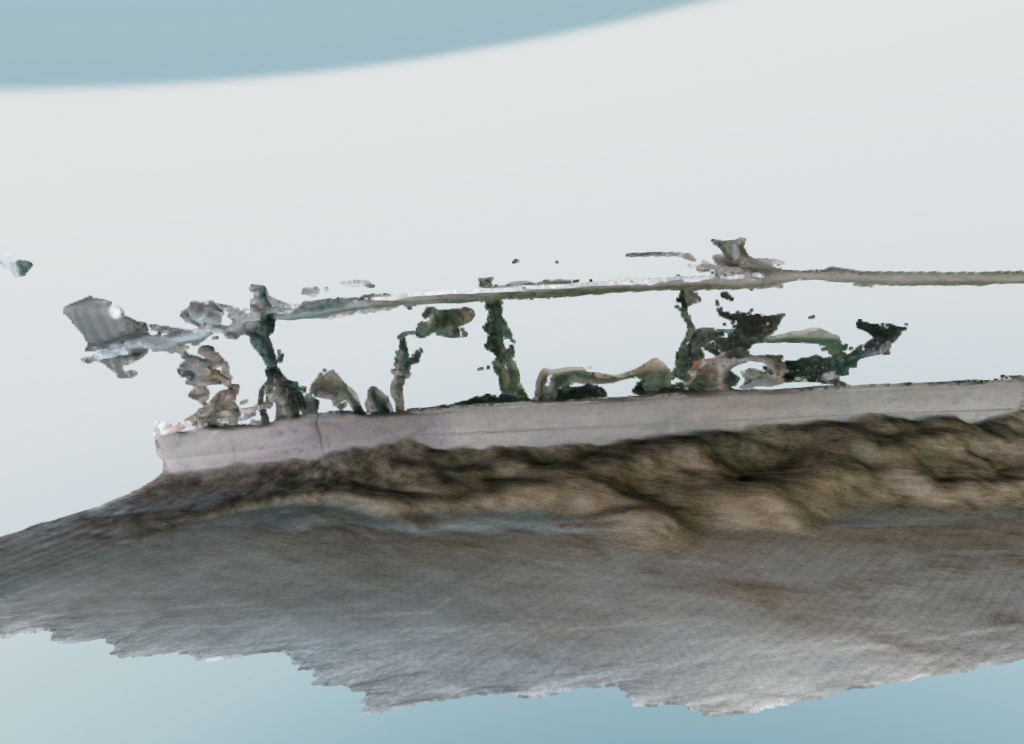
\includegraphics[width=\textwidth]{pics/recon_cow_maskout.png}
            \subcaption{Stall Rekonstruktion mithilfe von Segmentierungsmasken}
            \label{fig:recon_cow_maskout}
        \end{minipage}
        \hfill
        \begin{minipage}{0.45\textwidth}
            \centering
            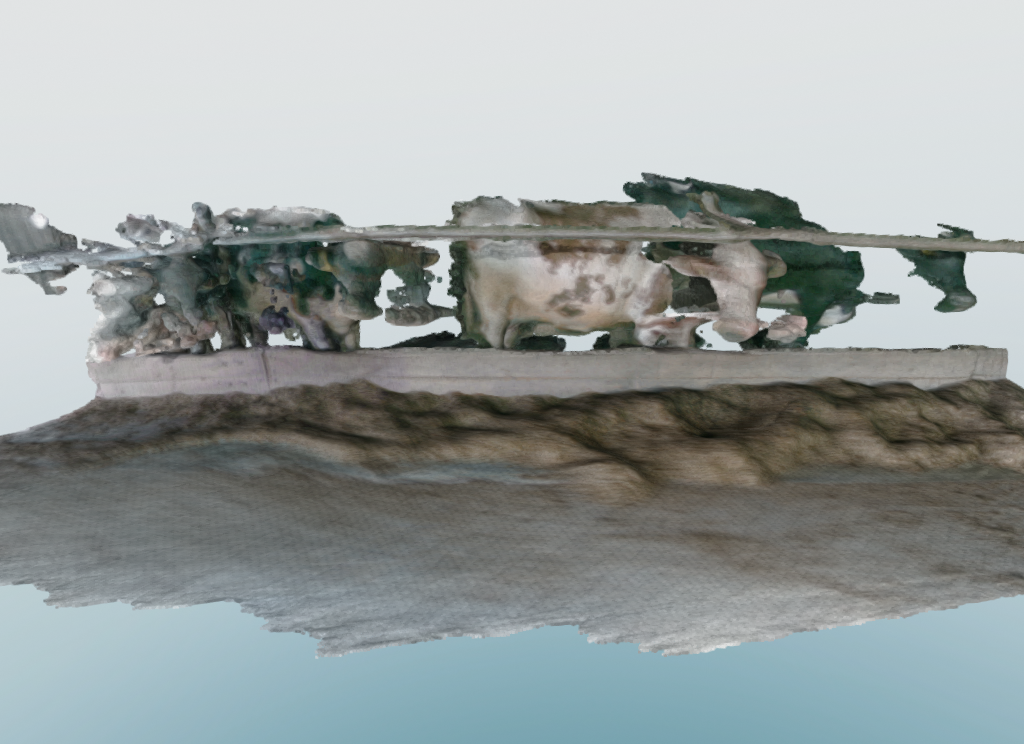
\includegraphics[width=\textwidth]{pics/recon_cow_raw.png}
            \label{fig:recon_cow_raw}
            \subcaption{Stall Rekonstruktion unmaskiert}
        \end{minipage}
        \caption{Stall Rekonstruktion ohne von Segmentierungsmasken}
        \label{fig:recon_cow}
    \end{figure}\noindent
    Im Fall der Futterstelle liegen keine konkreten Messdaten vor, die eine empirische Quantifizierung der Modellleistung erlauben würden. Dennoch kann die Rekonstruktion 
    betrachtet werden. Dafür wurden die Vorhersagen der Rohmasken direkt und ohne Post-Processing genutzt. \\\\
    In Abbildung \ref{fig:recon_cow} ist das Herausmaskieren der Kühe deutlich zu erkennen. Somit lassen sich die 
    Segmentierungsergebnisse teilweise in das Modell übertragen. Die Übertragung, sowie die schnelle Integration der Masken 
    in 3D-Szenen mittels Voxel-Block-Integration, eröffnet vielfältige Anwendungsmöglichkeiten.
    Die Kamerafahrt stammt aus demselben Stall, was die gute heraus Maskierung erklären kann. 
    \subsection{Zukunftiges Vorgehen}
    Die vorgestellte Testkonfiguration sowie die bisherigen Ergebnisse sind als vorläufig zu betrachten. 
    Eine detaillierte Analyse der Hyperparameterkonfiguration und des Verhaltens des Optimierers konnte bislang noch nicht in ausreichendem 
    Umfang durchgeführt werden. Weitere Testläufe mit unterschiedlichen Hyperparametern stehen noch aus. Zudem bietet sich eine Erweiterung der Experimente 
    auf verschiedene Backbone-Modelle unmittelbar an, was im weiteren Verlauf eingehender untersucht wird. \\\\
    Ein weiterer zentraler Aspekt betrifft den Datensatz: Eine stärkere Diversifizierung ist notwendig, um Trainings- und Validierungsdaten klarer voneinander 
    zu trennen und so eine bessere Übertragbarkeit der Ergebnisse auf andere Szenarien zu gewährleisten.\\\\    
    Die Verbindung mit der gezielten Integration von Masken führt unmittelbar zur 3D-Segmentierung. Eine genauere Betrachtung anhand gelabelter 
    3D-Daten bietet sich dabei an. In diesem Kontext erscheint auch der Einsatz stärker angepasster Integrationsverfahren vielversprechend.

    \chapter{Fazit und Ausblick}
    Das Ziel der Arbeit war es, ausgewählte Rekonstruktions- und Tracking-Algorithmen im Kontext von Stallumgebungen zu verbessern.
    Hierfür wurden die Verfahren der visuellen Odometrie sowie des \ac{TSDF}-Trackings durch die Einbeziehung von Masken erweitert.
    Die Anpassungen führten insbesondere in dynamischen Umgebungen zu deutlichen Verbesserungen. Besonders hervorzuheben ist dabei das 
    \ac{TSDF}-Tracking in Kombination mit dem Point-to-Point-Fehler und der Maskierung, das insgesamt robustere Ergebnisse erzielen konnte.\\\\
    Als nächster potenzieller Schritt erscheint die Betrachtung von Methoden zur Fusion mehrerer Tracking-Ansätze sinnvoll, um das \ac{TSDF}-Tracking 
    weiter zu stabilisieren und langfristig zu robustifizieren. Eine fortbestehende Herausforderung liegt dabei in der Szenenerfassung bei langen 
    Kameraverläufen. Aufgrund der baulichen Struktur des Stalls stehen nur wenige stabile Referenzpunkte über die Zeit zur Verfügung, was zu einer 
    Krümmung der rekonstruierten Szenen führen kann.\\\\
    Ein zweiter Schwerpunkt der Arbeit war die automatische Erstellung geeigneter Masken durch ein trainiertes Segmentierungsmodell. Die Segmentierung 
    lieferte adäquate Resultate durch das grobe Erkennen von Kühen und ermöglicht somit eine partielle Entfernung ihres Einflusses auf die 
    Rekonstruktionsmodelle. \\\\
    Für die Segmentierung ergibt sich als weiterer Arbeitsschritt die Diversifizierung des Datensatzes, um die Ergebnisse auf andere Umgebungen übertragen 
    zu können. Weitere und Umfangreiche Test-Experimente sind noch nötig um die letztendliche Performance zu verbessern.

    \clearpage
    \appendix

    \chapter{Anhang}
    \section{Hilfsmittel}
    Teile der sprachlichen Ausformulierung wurden mit Unterstützung des KI-Tools ChatGPT (OpenAI) erstellt. Inhaltliche Entscheidungen, Strukturierung, Methodik
    und wissenschaftliche Argumentation stammen jedoch vom Autor.
    \section{Rohdaten}
    \begin{landscape}
    \begin{table}[ht]
        \centering
        \caption{RPE visuelle Odoemtrie Multiscale 3 Pyramiden Level per 10 Iterationen}
        \label{tab:RPE_odom_eval}
        \setlength{\tabcolsep}{5pt} 
        \renewcommand{\arraystretch}{1.3}
        \resizebox{1.4\textwidth}{!}{
            \begin{tabular}{l*{10}{c}}
\toprule
    \multirow{2}{*}{\textbf{Methode}} & \multicolumn{2}{c}{\textbf{static xyz}} & \multicolumn{2}{c}{\textbf{static rpy}} & \multicolumn{2}{c}{\textbf{walking static}} & \multicolumn{2}{c}{\textbf{walking xyz}} & \multicolumn{2}{c}{\textbf{walking rpy}} \\
\cmidrule(lr){2-3}  \cmidrule(lr){4-5}  \cmidrule(lr){6-7}  \cmidrule(lr){8-9}  \cmidrule(lr){10-11}
    & \textbf{Trans. [m]} & \textbf{Rot. [rad]} & \textbf{Trans. [m]} & \textbf{Rot. [rad]} & \textbf{Trans. [m]} & \textbf{Rot. [rad]} & \textbf{Trans. [m]} & \textbf{Rot. [rad]} & \textbf{Trans. [m]} & \textbf{Rot. [rad]} \\
\midrule
Intensität  & 0.0222 & 0.0206 & 0.0199 & 0.0700 & 0.0156 & 0.0090 & 0.0302 & 0.0214 & 0.0308 & 0.0390 \\
Intensität maskiert & 0.0223 & 0.0206 & 0.0209 & 0.0706 & 0.0078 & 0.0079 & 0.0211 & 0.0205 & 0.0328 & 0.0399 \\
Hybrid  & 0.0232 & 0.0217 & 0.0227 & 0.0761 & 0.0126 & 0.0086 & 0.0294 & 0.0200 & 0.0281 & 0.0329 \\
Hybrid maskiert & 0.0232 & 0.0217 & 0.0230 & 0.0769 & 0.0066 & 0.0076 & 0.0189 & 0.0194 & 0.0245 & 0.0352 \\
P2P  & 0.0225 & 0.0213 & 0.0105 & 0.0883 & 0.0102 & 0.0073 & 0.0265 & 0.0175 & 0.0230 & 0.0367 \\
P2P maskiert & 0.0225 & 0.0213 & 0.0105 & 0.0883 & 0.0050 & 0.0064 & 0.0188 & 0.0171 & 0.0208 & 0.0359 \\
\bottomrule
\end{tabular}

        }
    \end{table}
    \begin{table}[ht]
        \centering
        \caption{ATE visuelle Odoemtrie 3 Pyramiden Level per 10 Iterationen}
        \label{tab:ATE_odom_eval}
        \setlength{\tabcolsep}{5pt} 
        \renewcommand{\arraystretch}{1.3}
        \resizebox{1.4\textwidth}{!}{
            \begin{tabular}{l*{10}{c}}
\toprule
    \multirow{2}{*}{\textbf{Methode}} & \multicolumn{2}{c}{\textbf{static xyz}} & \multicolumn{2}{c}{\textbf{static rpy}} & \multicolumn{2}{c}{\textbf{walking static}} & \multicolumn{2}{c}{\textbf{walking xyz}} & \multicolumn{2}{c}{\textbf{walking rpy}} \\
\cmidrule(lr){2-3}  \cmidrule(lr){4-5}  \cmidrule(lr){6-7}  \cmidrule(lr){8-9}  \cmidrule(lr){10-11}
    & \textbf{Trans. [m]} & \textbf{Rot. [rad]} & \textbf{Trans. [m]} & \textbf{Rot. [rad]} & \textbf{Trans. [m]} & \textbf{Rot. [rad]} & \textbf{Trans. [m]} & \textbf{Rot. [rad]} & \textbf{Trans. [m]} & \textbf{Rot. [rad]} \\
\midrule
Intensität  & 0.4480 & 0.4976 & 0.4733 & 1.3482 & 0.6179 & 0.2808 & 1.4618 & 0.6426 & 1.6596 & 1.2408 \\
Intensität maskiert & 0.4425 & 0.4686 & 0.7497 & 1.3497 & 0.3292 & 0.2123 & 0.6265 & 0.3568 & 1.4056 & 1.1543 \\
Hybrid  & 0.5359 & 0.4932 & 1.6487 & 2.0307 & 0.4870 & 0.2723 & 1.5046 & 0.7136 & 1.7352 & 1.1641 \\
Hybrid maskiert & 0.5273 & 0.4811 & 1.6585 & 2.0124 & 0.2554 & 0.2015 & 0.5800 & 0.3681 & 1.1007 & 1.0712 \\
P2P  & 0.5836 & 0.3370 & 0.3117 & 1.8171 & 0.4192 & 0.4001 & 2.7121 & 0.7409 & 1.3975 & 1.3223 \\
P2P maskiert & 0.5821 & 0.3400 & 0.3360 & 1.8257 & 0.3190 & 0.3884 & 1.2506 & 0.4905 & 0.7510 & 1.1356 \\
\bottomrule
\end{tabular}

        }
    \end{table}

    \end{landscape}
    
        \begin{landscape}
        \begin{table}[ht]
        \centering
        \caption{RPE TSDF-Tracking mit 3 Pyramiden Level per 10 Iterationen und gewichteter Integration}
        \label{tab:RPE_tsdf_eval}
        \setlength{\tabcolsep}{5pt} 
        \renewcommand{\arraystretch}{1.7}
        \resizebox{1.4\textwidth}{!}{
            \begin{tabular}{l*{10}{c}}
\toprule
    \multirow{2}{*}{\textbf{Methode}} & \multicolumn{2}{c}{\textbf{static xyz}} & \multicolumn{2}{c}{\textbf{static rpy}} & \multicolumn{2}{c}{\textbf{walking static}} & \multicolumn{2}{c}{\textbf{walking xyz}} & \multicolumn{2}{c}{\textbf{walking rpy}} \\
\cmidrule(lr){2-3}  \cmidrule(lr){4-5}  \cmidrule(lr){6-7}  \cmidrule(lr){8-9}  \cmidrule(lr){10-11}
    & \textbf{Trans. [m]} & \textbf{Rot. [rad]} & \textbf{Trans. [m]} & \textbf{Rot. [rad]} & \textbf{Trans. [m]} & \textbf{Rot. [rad]} & \textbf{Trans. [m]} & \textbf{Rot. [rad]} & \textbf{Trans. [m]} & \textbf{Rot. [rad]} \\
\midrule
Intensität default & $0.0212\pm 7.96\%$ & $0.0195\pm 6.34\%$ & $0.0184\pm 7.47\%$ & $0.0474\pm 0.83\%$ & $0.0124\pm 3.66\%$ & $0.0065\pm 1.41\%$ & $0.0879\pm 25.90\%$ & $0.0323\pm 21.51\%$ & $\textbf{--}$ & $\textbf{--}$ \\
Intensität maskiert & $0.0209\pm 3.64\%$ & $0.0194\pm 2.68\%$ & $0.0180\pm 3.27\%$ & $0.0471\pm 0.68\%$ & $0.0165\pm 19.65\%$ & $0.0075\pm 10.14\%$ & $0.0940\pm 37.86\%$ & $0.0343\pm 34.52\%$ & $\textbf{--}$ & $\textbf{--}$ \\
Hybrid default & $0.0115\pm 1.12\%$ & $0.0144\pm 0.36\%$ & $0.0318\pm 6.39\%$ & $0.0470\pm 2.81\%$ & $0.0101\pm 12.80\%$ & $0.0061\pm 5.66\%$ & $0.0287\pm 9.87\%$ & $0.0158\pm 3.96\%$ & $\textbf{--}$ & $\textbf{--}$ \\
Hybrid maskiert & $0.0114\pm 0.58\%$ & $0.0144\pm 0.24\%$ & $0.0329\pm 7.02\%$ & $0.0486\pm 4.72\%$ & $0.0075\pm 1.26\%$ & $0.0056\pm 0.68\%$ & $0.0280\pm 2.91\%$ & $0.0141\pm 1.17\%$ & $\textbf{--}$ & $\textbf{--}$ \\
P2P default & $0.0044\pm 0.04\%$ & $0.0109\pm 0.02\%$ & $0.0075\pm 0.07\%$ & $0.0201\pm 0.02\%$ & $0.0181\pm 7.50\%$ & $0.0094\pm 6.75\%$ & $0.0296\pm 9.46\%$ & $0.0177\pm 7.61\%$ & $\textbf{--}$ & $\textbf{--}$ \\
P2P maskiert & $0.0045\pm 0.05\%$ & $0.0109\pm 0.02\%$ & $0.0078\pm 0.08\%$ & $0.0201\pm 0.03\%$ & $0.0041\pm 0.22\%$ & $0.0057\pm 0.03\%$ & $0.0079\pm 0.52\%$ & $0.0126\pm 0.04\%$ & $0.0611\pm 51.08\%$ & $0.0399\pm 62.34\%$ \\
\bottomrule
\end{tabular}

        }
    \end{table}
    \begin{table}[ht]
        \centering
        \caption{ATE  TSDF-Tracking mit 3 Pyramiden Level per 10 Iterationen und gewichteter Integration}
        \label{tab:ATE_tsdf_eval}
        \setlength{\tabcolsep}{5pt} 
        \renewcommand{\arraystretch}{1.7}
        \resizebox{1.4\textwidth}{!}{
            \begin{tabular}{l*{10}{c}}
\toprule
    \multirow{2}{*}{\textbf{Methode}} & \multicolumn{2}{c}{\textbf{static xyz}} & \multicolumn{2}{c}{\textbf{static rpy}} & \multicolumn{2}{c}{\textbf{walking static}} & \multicolumn{2}{c}{\textbf{walking xyz}} & \multicolumn{2}{c}{\textbf{walking rpy}} \\
\cmidrule(lr){2-3}  \cmidrule(lr){4-5}  \cmidrule(lr){6-7}  \cmidrule(lr){8-9}  \cmidrule(lr){10-11}
    & \textbf{Trans. [m]} & \textbf{Rot. [rad]} & \textbf{Trans. [m]} & \textbf{Rot. [rad]} & \textbf{Trans. [m]} & \textbf{Rot. [rad]} & \textbf{Trans. [m]} & \textbf{Rot. [rad]} & \textbf{Trans. [m]} & \textbf{Rot. [rad]} \\
\midrule
Intensität default & $1.0399\pm 18.94\%$ & $0.6811\pm 21.08\%$ & $0.6808\pm 16.23\%$ & $1.0558\pm 12.88\%$ & $0.0683\pm 3.91\%$ & $0.0215\pm 3.68\%$ & $2.7599\pm 33.63\%$ & $1.0619\pm 52.83\%$ & $\textbf{--}$ & $\textbf{--}$ \\
Intensität maskiert & $1.2910\pm 32.83\%$ & $0.9918\pm 26.01\%$ & $0.7712\pm 9.00\%$ & $1.0139\pm 14.92\%$ & $0.0425\pm 25.70\%$ & $0.0173\pm 13.49\%$ & $2.8556\pm 31.88\%$ & $1.1483\pm 56.38\%$ & $\textbf{--}$ & $\textbf{--}$ \\
Hybrid default & $0.0578\pm 2.17\%$ & $0.1179\pm 1.29\%$ & $1.0401\pm 38.40\%$ & $0.8918\pm 20.38\%$ & $0.1712\pm 87.18\%$ & $0.0543\pm 83.24\%$ & $2.0014\pm 24.41\%$ & $0.9059\pm 14.65\%$ & $\textbf{--}$ & $\textbf{--}$ \\
Hybrid maskiert & $0.0544\pm 1.36\%$ & $0.1178\pm 0.72\%$ & $1.0982\pm 43.08\%$ & $0.9033\pm 19.95\%$ & $0.0310\pm 1.87\%$ & $0.0150\pm 0.77\%$ & $0.2893\pm 3.71\%$ & $0.0655\pm 17.25\%$ & $\textbf{--}$ & $\textbf{--}$ \\
P2P default & $0.0330\pm 0.03\%$ & $0.0336\pm 0.02\%$ & $0.0766\pm 0.10\%$ & $0.1021\pm 0.02\%$ & $0.8969\pm 19.69\%$ & $0.2534\pm 35.27\%$ & $1.2095\pm 17.29\%$ & $0.8985\pm 10.30\%$ & $\textbf{--}$ & $\textbf{--}$ \\
P2P maskiert & $0.0329\pm 0.02\%$ & $0.0336\pm 0.02\%$ & $0.0759\pm 0.07\%$ & $0.1022\pm 0.02\%$ & $0.0466\pm 0.03\%$ & $0.0136\pm 0.04\%$ & $0.1053\pm 0.05\%$ & $0.0320\pm 0.05\%$ & $1.1831\pm 56.88\%$ & $0.8706\pm 75.58\%$ \\
\bottomrule
\end{tabular}

        }
    \end{table}
    \end{landscape}
    \printbibliography 
    \eigenstaenigkeitserklaerung

    \cleardoublepage

    \pagenumbering{roman}


\end{document}
